\documentclass[aps,preprintnumbers,showpacs,nofootinbib,superscriptaddress,floatfix]{revtex4}

\pdfoutput=1 % if your are submitting a pdflatex (i.e. if you have
             % images in pdf, png or jpg format)

%%%%%%%%%%%%%%%%%%%%%%%%%%%%
\usepackage{graphicx}
\usepackage{amssymb}
\usepackage{amsmath}
\usepackage{bm}
\usepackage{slashed}
\usepackage{datetime}
\usepackage{mciteplus}
\usepackage{multirow}
\usepackage{color}

%%%%%%%%%%%%%%%%%%%%%%%%%%%

\newcommand{\xbj}{x_B}
\newcommand{\zh}{z_h}

%% macro to draw particularly short right arrows. Choose one of the two
\newcommand{\smarrow}{\mbox{\raisebox{-4.5pt}[0pt][0pt]{$\hspace{-1pt} 
		\vec{\phantom{v}}$}}}
%\newcommand{\smarrow}{\mbox{\raisebox{0.5pt}{\tiny $\hspace{-1.5pt} \rightarrow 
%\hspace{-8.25pt}{\color{white} \rule[1pt]{1.5pt}{0.5pt}} \hspace{4pt} $}} }

%% names of experiments + MINUIT
\newcommand{\hermes}{\textsc{Hermes }}
\newcommand{\compass}{\textsc{Compass }}
\newcommand{\minuit}{\textsc{Minuit }}

%% macro to manage T versus perp notation
\newcommand{\T}{\perp}
\newcommand{\Tperp}{T}
\newcommand{\bT}{\zeta_T}

%%%%%%%%%%%%%%%%%%%%%%%%%%%%%%%%%%%%%%%%%%%%%%%

\begin{document}
\allowdisplaybreaks[2]


\title{
Extraction of partonic transverse momentum distributions 
from semi-inclusive deep
inelastic scattering and Drell-Yan data
}

\author{Alessandro Bacchetta}
\email{alessandro.bacchetta@unipv.it}
\affiliation{Dipartimento di Fisica, Universit\`a di Pavia, via Bassi 6,
  I-27100 Pavia} 
\affiliation{INFN Sezione di Pavia, via Bassi 6, I-27100 Pavia, Italy}

\author{Filippo Delcarro}
\email{filippo.delcarro01@ateneopv.it}
\affiliation{Dipartimento di Fisica, Universit\`a di Pavia, via Bassi 6,
  I-27100 Pavia} 
\affiliation{INFN Sezione di Pavia, via Bassi 6, I-27100 Pavia, Italy}

\author{Cristian Pisano}
\email{alessandro.bacchetta@unipv.it}
\affiliation{Dipartimento di Fisica, Universit\`a di Pavia, via Bassi 6,
  I-27100 Pavia} 
\affiliation{INFN Sezione di Pavia, via Bassi 6, I-27100 Pavia, Italy}

\author{Marco Radici}
\email{marco.radici@pv.infn.it}
\affiliation{INFN Sezione di Pavia, via Bassi 6, I-27100 Pavia, Italy}

\author{Andrea Signori}
\email{asignori@jlab.org}
\affiliation{Theory Center, Thomas Jefferson National Accelerator Facility, 12000 Jefferson Avenue, Newport News, VA 23606, USA}
\affiliation{Department of Physics and Astronomy, VU University Amsterdam, De
  Boelelaan 1081, NL-1081 HV Amsterdam, the Netherlands}
\affiliation{Nikhef, Science Park 105, NL-1098 XG Amsterdam, the
  Netherlands}

\begin{abstract}
We present an extraction of unpolarized partonic transverse momentum
distributions (TMDs) 
from a simultaneous fit of available data measured in semi-inclusive deep inelastic scattering 
and in Drell-Yan processes through the production of photon and $Z$ bosons. 
To connect data at different scales, we use TMD evolution at next-to-leading logarithmic accuracy. The
analysis is restricted to the low-transverse-momentum region, with no matching
to fixed-order calculations at high transverse momentum. We introduce specific
choices to deal with TMD evolution at low scales, of the order of 1 GeV$^2$.
This could be considered as a first attempt at a global fit of TMDs.
\end{abstract}

\preprint{JLAB THY 17-****}

\date{\today, \currenttime}

\pacs{13.60.Le, 13.87.Fh,14.20.Dh}

\maketitle

%%%%%%%%%%%%%%%%%%%%%%%%%%%%%%%%%%%%%%%%%%%%%%%%%%%%%%%%%%%%%%%%%%
\section{Introduction}
\label{s:intro}
%%%%%%%%%%%%%%%%%%%%%%%%%%%%%%%%%%%%%%%%%%%%%%%%%%%%%%%%%%%%%%%%%%

Parton distribution functions describe the internal structure of the nucleon
in terms of its elementary constituents (quarks and gluons). They cannot be
easily computed from first principles, because they require the ability to
carry out Quantum Chromodynamics (QCD) calculations in a nonperturbative
regime. Many experimental observables in hard scattering experiments
involving hadrons are related to parton distribution functions (PDFs) and
fragmentation functions (FFs), in a way that is specified by factorization
theorems (see, e.g., Refs.~\cite{Collins:1989gx,Collins:2011zzd}). 
These theorems also elucidate the universality properties of PDFs and FFs
(i.e., the fact that they are the same in different processes) 
and their evolution equations (i.e., how they get modified by the change in
the hard scale of the process). 
Availability of measurements of different processes in different
experiments makes it possible to test the reliability of factorization
theorems and extract PDFs and FFs through so-called global fits. 
On the other side, the knowledge of PDFs and FFs allows us
to make predictions for other hard hadronic processes. 
These general statements apply equally well to
standard collinear PDFs and FFs and to transverse-momentum-dependent parton
distribution functions (TMD PDFs) and fragmentation functions (TMD FFs). 
Collinear PDFs
describe the distribution of partons integrated over all components of
partonic momentum except the one collinear to the parent hadron; hence,
collinear PDFs
are functions only of the parton longitudinal momentum fraction $x$. 
TMD PDFs (or TMDs for short) 
include also the dependence on transverse momentum components $k_{\T}^2$. 
They can be interpreted as three-dimensional generalizations of collinear PDFs.
Similar arguments apply to collinear FFs and TMD FFs.

There are several differences between collinear and TMD distributions. From
the formal point of view, factorization theorems for the two types of
functions are qualitatively different, implying also different universality
properties and evolution equations~\cite{Rogers:2015sqa}. From the
experimental point 
of view, observables related to TMDs require the measurement of some transverse
momentum component much smaller than the hard scale of the
process~\cite{Bacchetta:2016ccz,Radici:2016hbh}.  For
instance, Deep-Inelastic Scattering (DIS) is characterized by a hard scale represented by the
4-momentum squared of the virtual photon ($-Q^2$). In inclusive DIS this is
the only scale of the process, and access is limited to collinear PDFs
and FFs. In semi-inclusive DIS (SIDIS) also the transverse momentum of the
outgoing  
hadron ($P_{hT}$) can be measured~\cite{Mulders:1995dh,Bacchetta:2006tn}. 
If $P_{hT}^2\ll Q^2$, TMD
factorization can be applied and the process is sensitive to
TMDs~\cite{Collins:2011zzd}. 

%If $P_{h\perp}^2\sim Q^2$ or if the measurement is integrated over $P_{h\perp}$,
%collinear factorization applies and the process is sensitive to collinear
%PDFs. 

If polarization is taken into account, several TMDs can be
introduced~\cite{Mulders:1995dh,Boer:1997nt,%quark twist 2, spin 1/2
Bacchetta:2000jk,%quark twist 2, spin 1
Mulders:2000sh,%gluon twist 2, spin 1/2
Boer:2016xqr%gluon twist 2, spin 1
}. Attempts to extract some of them have already been presented in the past~\cite{Bacchetta:2011gx,Anselmino:2012aa,Echevarria:2014xaa,Anselmino:2016uie,%Sivers
Lu:2009ip,Barone:2015ksa,%Boer-Mulders
Lefky:2014eia,%pretzelosity
Anselmino:2013vqa,Kang:2015msa%Collins
}.  In
this work, we focus on the simplest ones, i.e., the unpolarized TMD
PDF $f_1^q(x,k_{\T}^2)$ and the unpolarized TMD
FF $D_1^{q \to h}(z,P_{hT}^2)$, where $z$ is
  the fractional energy carried by the detected hadron $h$. Despite their
  simplicity, the phenomenology of these unpolarized TMDs present several
  challenges~\cite{Signori:2016lvd}: the functional form of TMDs at low
  partonic transverse momentum, its possible dependence on the parton
  flavor~\cite{Signori:2013mda}, the implementation of TMD
  evolution~\cite{Bacchetta:2015ora,Rogers:2015sqa}, the matching to
  fixed-order calculations in collinear
  factorization~\cite{Collins:2016hqq}. 

We take into consideration three kinds of processes: semi-inclusive DIS, and
Drell--Yan processes (DY) with the production of virtual photons and $Z$
bosons. To date, they represent \textcolor{red}{almost [AB:why almost? what
  else could be used?]} all possible processes
  where experimental information is available for unpolarized TMD
  extractions. 
The only important
process currently missing is electron-positron annihilation, which is
particularly important for the determination of TMD
FFs~\cite{Bacchetta:2015ora}. This work can therefore be considered as the
first attempt at a global fit of TMDs.  

The paper is organized as follows. In Sec.~\ref{s:theory}, the general
formalism for TMDs in SIDIS and DY processes is briefly outlined, including a
description of the assumptions and approximations in the phenomenological
implementation of TMD evolution equations. In Sec.~\ref{s:data}, the criteria
for selecting the data analyzed in the fit are summarized and commented. In
Sec.~\ref{s:results}, the results of our global fit are presented and
discussed. In Sec.~\ref{s:end}, we draw some conclusions. 
   

%%%%%%%%%%%%%%%%%%%%%%%%%%%%%%%%%%%%%%%%%%%%%%%%%%%%%%%%%%%%%%%%%%
\section{Formalism}
\label{s:theory}
%%%%%%%%%%%%%%%%%%%%%%%%%%%%%%%%%%%%%%%%%%%%%%%%%%%%%%%%%%%%%%%%%%

\textcolor{blue}{Shall we add pictures for the kinematics of SIDIS and DY data ? E.g. see Fig. 1 in~\cite{Signori:2013mda}.}

%%%%%%%%%%%%%%%%%%%%%%%%%%%%%%%%%%%%
\subsection{Semi-inclusive DIS}
\label{ss:SIDIS_formalism}

In one-particle \textcolor{red}{SIDIS}, a lepton $\ell$ with momentum $l$ scatters 
off a hadron target $N$ with mass $M$ and momentum
$P$. In the final state, the scattered lepton momentum 
$l'$ is measured together with
one hadron $h$ with mass $M_h$
and momentum $P_h$. The corresponding reaction formula is  
\begin{equation}
  \label{e:sidis}
\ell(l) + N(P) \to \ell(l') + h(P_h) + X \, .
\end{equation}
The space-like momentum transfer is $q = l - l'$, with $Q^2 = - q^2$. We
introduce the usual invariants  
\begin{align}
  \label{e:xyz}
x &= \frac{Q^2}{2\,P\cdot q},
&
y &= \frac{P \cdot q}{P \cdot l},
&
z &= \frac{P \cdot P_h}{P\cdot q},
&
\gamma &= \frac{2 M x}{Q} .
\end{align}

The available data refer to \textcolor{red}{SIDIS} hadron multiplicities, namely to the differential number of hadrons produced per corresponding inclusive DIS event. In terms of cross sections, we define the multiplicities as
\begin{equation}
m_N^h (x,z,|\bm{P}_{h\Tperp}|, Q^2) = \frac{d \sigma_N^h / ( dx  dz d|\bm{P}_{h\Tperp}| dQ^2) }
                                                                   {d\sigma_{\text{DIS}} / ( dx dQ^2 ) }\, ,
\label{e:multiplicity}
\end{equation}
where $d\sigma_N^h$ is the differential cross section for the \textcolor{red}{SIDIS} process and $d\sigma_{\text{DIS}}$ is the corresponding inclusive one, 
and where \( \bm{P}_{h\Tperp} \) is the component of \( \bm{P}_{h} \) transverse to \( \bm{q} \). 
In the single-photon-exchange approximation, the multiplicities can be written as ratios of
structure functions (see \cite{Bacchetta:2006tn} for details):
\begin{equation}
m_N^h (x,z,|\bm{P}_{h\Tperp}|, Q^2) =   
\frac{2 \pi\,|\bm{P}_{h\Tperp}| F_{UU ,T}(x,z,\bm{P}_{h\Tperp}^2, Q^2) + 2 \pi
  \varepsilon |\bm{P}_{h\Tperp}| F_{UU ,L}(x,z,\bm{P}_{h\Tperp}^2, Q^2)}
        {F_{T}(x,Q^2) + \varepsilon  F_{L}(x,Q^2)} \, ,
 \label{e:mFF}
\end{equation} 
where
\begin{align}
\varepsilon &= \frac{1-y -\frac{1}{4} \gamma^2 y^2}{1-y+\frac{1}{2} y^2 +\frac{1}{4} \gamma^2 y^2} \ ,
\end{align}  
\textcolor{red}{and the structure function $F_{XY,Z}$ corresponds to a lepton with polarization $X$ scattering on a target with polarization $Y$ by exchanging a virtual photon in a polarization state $Z$.}

The semi-inclusive cross section can be expressed in a factorized form in terms of TMDs only in the kinematical limits $M^2 \ll Q^2$ and $\bm{P}_T^2 \ll Q^2$. In these limits, the structure function $F_{UU,L}$ of Eq.~\eqref{e:mFF} can be neglected~\cite{Bacchetta:2008xw}. The structure function $F_L$ in the denominator contains contributions involving powers of the strong coupling constant $\alpha_S$ at an order that goes beyond the level reached in this analysis; hence, it will be consistently neglected (see also Ref.~\cite{Signori:2013mda}).

To express the structure functions in terms of TMD PDFs and FFs, 
we rely on the factorized formula 
for \textcolor{red}{SIDIS}~\cite{Collins:1981uk,Collins:1984kg,Ji:2002aa,Ji:2004wu,%
Collins:2011zzd,Aybat:2011zv,GarciaEchevarria:2011rb,Echevarria:2012pw,%
Collins:2012uy}:  
\begin{align}
\label{e:SIDISkT}
   F_{UU,T}(x,z, \bm{P}_{h \Tperp}^2, Q^2) &= \sum_a \mathcal{H}_{UU,T}^{a}(Q^2;\mu^2) \\ 
      &\times \int d\bm{k}_\T^{} \, d\bm{P}_\T^{} \,  f_1^a\big(x,\bm{k}_{\T}^2; \mu^2 \big) \, D_{1}^{a\smarrow h}\big(z,\bm{P}_{\T}^2; \mu^2 \big) \,
      \delta \big(z {\bm k}_{\T} - {\bm P}_{h \Tperp} + {\bm P}_{\T}\big)
\nonumber\\&
\nonumber + Y_{UU,T}\big(Q^2, \bm{P}_{h\Tperp}^2\big) + \mathcal{O}\big(M^2/Q^2\big) \, .
\end{align} 
Here, $\mathcal{H}_{UU,T}$ is the hard scattering part; $f_1^a(x,\bm{k}_{\T}^2;
\mu^2)$ is the TMD distribution of unpolarized partons with flavor $a$ in an unpolarized
proton, carrying longitudinal momentum fraction $x$ and transverse momentum
$\bm{k}_\T$ at the factorization scale $\mu^2$, which in the following we
choose to be equal to $Q^2$.  The $D_1^{a\smarrow h}(z, \bm{P}_{\T}^2;
\mu^2)$ is the TMD fragmentation function describing the fragmentation of an unpolarized parton with flavor $a$ into
an unpolarized hadron $h$ carrying longitudinal momentum fraction $z$ and
transverse momentum 
$\bm{P}_\T$. The term $Y_{UU,T}$ is introduced to ensure a matching
to the perturbative fixed-order calculations at higher transverse momenta. 

The applicability of Eq.~\eqref{e:SIDISkT} 
relies on the possibility of
neglecting $M^2/Q^2$ corrections.
At large $Q^2$ this should not pose serious
problems. However, fixed-target DIS experiments typically 
collect a large amount of data
at relatively low $Q^2$ values, which may lead to problems (see, e.g., recent
discussions in Refs.~\cite{Boglione:2016bph,Moffat:2017sha}).

 

Eq.~\eqref{e:SIDISkT} can be expanded in powers
of $\alpha_S$. In the present analysis, we 
will consider only the leading order terms in $\alpha_S$, i.e., stop at
order $\alpha_S^0$. In this case $\mathcal{H}_{UU,T} (Q^2, \mu^2) \approx 1$
and $Y_{UU,T}\approx 0$. 
However, perturbative corrections include large logarithms $L \equiv
\log\big(z^2 Q^2/P_{hT}^2\big)$, so that $\alpha_S L \approx 1$.
In the present analysis, we will take into account all 
powers of the form $\alpha_S^n L^{2n} \approx 1$ (Leading Logarithms --LL) 
and 
$\alpha_S^n L^n \approx 1$ (Next-to-Leading Logarithms -- NNL).

In these approximations (LO in $alpha_S$ and NLL), only the first term in
Eq.~\eqref{e:SIDISkT} is relevant (often in the
literature this has been called $W$ term). We expect this term to provide a
good description of the
structure function only in the region where $P_{hT}^2/z^2 \ll Q^2$. 
It can happen that $Y_{UU,T}$, defined
in the standard way (see, e.g., Ref.~\cite{Collins:1984kg}), gives large
contributions also in this region, but it is admissible to
redefine it in order to avoid this problem~\cite{Collins:2016hqq}. 
We leave a detailed treatment of the matching to the high $P_{hT}^2 \approx Q^2$
region to future investigations.   

To the purpose of applying TMD evolution equations, 
 need to calculate the Fourier transform of the the part of 
Eq.~\eqref{e:SIDISkT} involving TMDs. The structure function thus reduces to 
\begin{align}
\label{e:SIDISkTFF}
   F_{UU,T}(x,z, \bm{P}_{h \Tperp}^2, Q^2) &\approx \sum_a  
      \int_0^{\infty} \frac{d \bT}{2 \pi} \bT J_0\big(\bT |\bm{P}_{hT}|/z\big)
      \tilde{f}_1^a\big(x, \bT;Q^2\big) \tilde{D}_1^{a\smarrow h}\big(z, \bT;
      Q^2 \big) 
\nonumber \, .
\end{align} 
\textcolor{red}{ E' questa la formula usata nel codice, o serve dire altro?}
where we introduced the Fourier transforms of the TMD PDF and FF according to
\begin{align} 
\tilde{f}_1^a\big(x, \bT;\mu^2\big) &=
% \int_0^{\infty} \frac{d^2 \bm{k}_\T}{(2 \pi)^2} e^{i \bm{k}_\T \cdot \bm{b}_T}
%       f_1^a\big(x, \bm{k}_\T^2;\mu^2\big)
%\\ &= 
\int_0^{\infty}\frac{d |\bm{k}_\T|}{2 \pi} 
                |\bm{k}_\T|J_0\big(\bT |\bm{k}_\T|\big) 
       f_1^a\big(x, \bm{k}_\T^2;\mu^2\big),
\\
\tilde{D}_1^{a\smarrow h}\big(z, \bT; \mu^2 \big) &=
%\int_0^{\infty} \frac{d^2 \bm{P}_\T}{(2 \pi)^2 z^2} e^{i (\bm{P}_\T \cdot \bm{b}_T)/z}
%       D_1^{a\smarrow h}\big(z, \bm{P}_{\T}^2; \mu^2 \big)
%\\ &=
 \int_0^{\infty} \frac{d |\bm{P}_{\T}|}{2 \pi z^2} |\bm{P}_{\T}| 
                                             J_0\big(\bT |\bm{P}_{\T}|/z\big)
       D_1^{a\smarrow h}\big(z, \bm{P}_{\T}^2; \mu^2 \big).
\end{align}  


%%%%%%%%%%%%%%%%%%%%%%%%%%%%%%%%%%%%
\subsection{Drell--Yan processes}
\label{ss:DY_formalism}

In a Drell--Yan process, two hadrons $A$ and $B$ with momenta $P_A$ and $P_B$
collide at a center-of-mass energy squared $s = (P_A + P_B)^2$ 
and produce a virtual photon or a $Z$ boson plus hadrons. 
The boson decays into a
lepton-antilepton pair. The reaction formula is
\begin{equation}
A(P_A)+B(P_B)\to [\gamma^*/Z + X \to] \ell^+(l) + \ell^-(l') + X.
\end{equation} 
The invariant mass of the virtual photon is $Q^2=q^2$ with $q = l + l'$. 
We introduce the rapidity of the virtual photon/Z boson
\begin{equation}
\eta=\frac{1}{2}\log\bigg(\frac{q^0+q_z}{q^0-q_z}\bigg)\  .
\end{equation} 
where the $z$ direction is defined along the momentum of hadron A.

The cross section can be written in terms of structure
functions~\cite{Boer:2006eq,Arnold:2008kf}. For our purposes, we need the unpolarized 
cross section
integrated over $d\Omega$ and over the azimuthal angle of the virtual photon, 
\begin{align}
\frac{d\sigma}{dQ^2\, dq_T^2\,d\eta} &= \sigma_0^{\gamma,Z}
\bigg(F_{UU}^1 + \frac{1}{2} F_{UU}^2\bigg). 
\end{align} 
The elementary cross sections are
\begin{align}
\sigma_0^{\gamma} &= \frac{4\pi \alpha^2_{\rm em}}{3 Q^2 s},
&
\sigma_0^Z &= 
%\frac{\sqrt{2} \pi G_F M_Z^2}{s}
\frac{\pi^2 \alpha_{\rm em}}{s (\sin^2{\theta_W} \cos^2{\theta_W}}
B_R(Z\rightarrow \ell^+\ell^-)
\delta(Q^2 - M_Z^2), 
\end{align} 
where $\theta_W$ is Weinberg's angle, $M_Z$ is the mass of the $Z$ boson, and
$B_R$ is the branching ratio for the $Z$ boson decay in two leptons.
We adopted the narrow-width approximation, i.e., we neglect contributions for 
$Q^2 \neq M_Z^2$. 
We used the values 
$\sin^2 \theta_W= 0.2313$, $M_Z = 91.18$ GeV, and 
$B_R(Z\rightarrow \ell^+\ell^-)=3.366$.  

\textcolor{red}{[ Secondo me nella prima delle eq.(10) ci vuole $\pi^2$. Infatti, partendo da Ref.[14] abbiamo}
\begin{align}
\frac{d\sigma}{d^4q} &= \frac{\alpha^2}{s Q^2}\, \frac{8 \pi}{3} \, \left[ F_{UU}^1 + \frac{1}{2}\, F_{UU}^2 \right] 
\nonumber
\end{align}
\textcolor{red}{Ora $d^4 q = dq^+ dq^- dq_x dq_y$. Lo Jacobiano della trasformazione $|| dQ^2 d\eta / dq^+ dq^- || = 2$. Mentre quello per $||dq_T^2 d\theta_q / dq_x dq_y|| = 2$. Quindi }
\begin{align}
\frac{d\sigma}{dQ^2 d\eta dq_T^2 d\theta_q} &= \frac{1}{4} \, \frac{d\sigma}{d^4q} = \frac{\alpha^2}{s Q^2}\, \frac{2 \pi}{3} \, \left[ F_{UU}^1 + \frac{1}{2}\, F_{UU}^2 \right] 
\nonumber
\end{align}
\textcolor{red}{L'ulteriore integrazione in $d\theta_q$ fornisce un $2\pi$, quindi}
\begin{align}
\frac{d\sigma}{dQ^2 d\eta dq_T^2} &= \frac{\alpha^2}{s Q^2}\, \frac{4 \pi^2}{3} \, \left[ F_{UU}^1 + \frac{1}{2}\, F_{UU}^2 \right] 
\nonumber
\end{align}
\textcolor{red}{Vi torna? ]
\textcolor{red}[AB: I started from Eq. 57 of Ref. \cite{Arnold:2008kf} and I
integrated over the solid angle. The integration over $\phi$ is trivial and
gives a $2 \pi$. The
integration over $cos\theta$ gives a factor $8/3$ in front of $F_{UU}^1$
 and a factor $4/3$ in front of $F_{UU}^2$. The $F$ factor in the
 denominator, neglecting hadron masses, is equal to $2s$ (see first line of p.
 3). Finally, there is the factor 2 in the denomininator coming from the first
 Jacobian of Marco. ]}

\textcolor{red}{Similarly to the SIDIS case, in the kinematical limit $q_T^2 \ll Q^2$ and neglecting the hadron masses the structure function $F_{UU}^2$ can be neglected.}
%Similar reasons as for the semi-inclusive DIS case leads us to neglecting
%the structure function $F_{UU}^2$.

The longitudinal momentum fractions can be written in terms of
rapidity in the following way 
\begin{align}
x_A &= \frac{Q}{\sqrt{s}} e^{\eta},
&
x_B &= \frac{Q}{\sqrt{s}} e^{-\eta}.
\label{xab}
\end{align} 
Some experiments use the variable $x_F$, which is connected to the other
variables  by the following relations
\begin{align}
\label{e:eta_xf}
\eta &= \sinh^{-1}\bigg(\frac{\sqrt{s}}{Q}\frac{x_F}{2}\bigg),
& 
x_{A} &= \sqrt{\frac{Q^2}{s} + \frac{x_F^2}{4}} + \frac{x_F}{2},
&
x_B &= x_A - x_F.  
\end{align} 

The structure function $F_{UU}^1$ can be written as
\begin{align}
\label{e:DYkT}
   F_{UU}^1(x_A,x_B, \bm{q}_{T}^2, Q^2) &= \sum_a \mathcal{H}_{UU}^{1 a}(Q^2;\mu^2) \\ 
      &\times \int d\bm{k}_{\T A}^{} \, d\bm{k}_{\T B}^{} 
\,  f_1^a\big(x_A,\bm{k}_{\T A}^2; \mu^2 \big) 
\, f_{1}^{\bar{a}}\big(x_B,\bm{k}_{\T B}^2; \mu^2 \big) \,
      \delta \big({\bm k}_{\T A} - {\bm q}_T + {\bm k}_{\T B}\big)
\nonumber\\&
\nonumber + Y_{UU}^1\big(Q^2, \bm{q}_T^2\big) + \mathcal{O}\big(M^2/Q^2\big) \, .
\end{align} 


\textcolor{red}{As in the SIDIS case, with the above kinematical limits the
  $Y_{UU}$ term and corrections from higher twists of order $M^2/Q^2$ or
  higher can be neglected.}
In our analysis, we consider the hard coefficients only up to leading order in
the couplings, i.e.,
\begin{align} 
{\cal H}_{UU, \gamma}^{1 a}(Q^2;\mu^2) &\approx \frac{e_a^2}{N_c},
&
{\cal H}_{UU, Z}^{1 a}(Q^2;\mu^2) &\approx \frac{V_a^2+A_a^2}{N_c} \ ,
\end{align}  
where\footnote{We remind the reader that the value of weak isospin $I_3$ is equal to $+1$ for $u$, $c$, $t$ and
  $-1$ for $d$, $s$, $b$.}
\begin{align}
V_a & = I_{3a} - 2 e_{a} \sin \theta_W \  ,
&
A_a & = I_{3a} \  .
\end{align} 

\textcolor{red}{The structure function can be conveniently expressed as a Fourier transform of the right-handside of Eq.~\eqref{e:DYkT} as }
\begin{align}
\label{e:DYkTFF}
   F_{UU}^1(x_A,x_B, \bm{q}_T^2, Q^2) &=
 \sum_a {\cal H}_{UU}^{1 a} \, \int_0^{\infty} \frac{d \bT}{2 \pi} \bT\, J_0\big( \bT |\bm{q}_T|\big)\ 
      \tilde{f}_1^a\big(x_A, \bT;\mu^2\big) \   \tilde{f}_1^{\bar{a}}\big(x_B, \bT;\mu^2 \big)  \, .
\end{align} 

\textcolor{red}{ Stessa osservazione che in SIDIS: \`e questa la formula usata nel codice, o serve dire altro?}



%%%%%%%%%%%%%%%%%%%%%%%%%%%%%%%%%%%%
\subsection{TMDs and their evolution}
\label{ss:TMDevo}

Following the formalism of Refs.~\cite{Collins:2011zzd,Aybat:2011zv}, the
unpolarized TMD distribution and fragmentation functions in configuration
space for a parton flavor $a$ at a certain scale $\mu^2$ can be written as 
\begin{align}   
\widetilde{f}_1^a (x,  \bT; \mu^2) &= \sum_{i=q,\bar q,g} \bigl( C_{a/i} \otimes f_1^i \bigr) (x; \mu_b^2) 
\  e^{S (\mu_b^2, \mu^2)} \  e^{g_K(\bT) \ln (\mu^2 / Q_0^2)} \  \widetilde{f}_{1 {\rm NP}}^a (x, \bT) \ ,
\label{e:TMDevol1} \\
\widetilde{D}_1^{a\to h} (z, \bT; \mu^2) &= \sum_{i=q,\bar q,g} \bigl( \hat{C}_{a/i} \otimes D_1^{i\to h} \bigr) (z; \mu_b^2) \  e^{S (\mu_b^2, \mu^2)} \  e^{g_K( \bT) \ln (\mu^2 / Q_0^2)} \  \widetilde{D}_{1 {\rm NP}}^{a\to h} (z, \bT) \  .
\label{e:TMDevol2}
\end{align}

The $C$ and $\hat{C}$ are perturbatively calculable Wilson coefficients for
the TMD distribution and fragmentation functions, respectively. They are
convoluted with the corresponding collinear functions according to 
\begin{align}
\bigl( C_{a/i} \otimes f_1^i \bigr) (x, \bar{b}_{\ast}; \mu_b^2) &=
  \int_x^1 \frac{du}{u}\  
        C_{a/i} \Big( \frac{x}{u}, \alpha_S\big(\mu_b^2\big)  \Big) \  
        f_1^i (u; \mu_b^2) \  , 
\label{e:WC1} \\
\bigl( \hat{C}_{a/i} \otimes D_1^{i\to h} \bigr) (z, \bar{b}_{\ast}; \mu_b^2) &= \int_z^1 \frac{du}{u}\  \hat{C}_{a/i} \left( \frac{z}{u}, \bar{b}_{\ast}; \mu_b^2 \right) \  D_1^{i\to h} (u; \mu_b^2) \  . 
\label{e:WC2}
\end{align}
In the present analysis, we consider only the leading-order term
in the $\alpha_S$ expansion, i.e., 
\begin{align} 
C_{a/i} \Big( \frac{x}{u}, \alpha_S\big(\mu_b^2\big)  \Big) &\approx
\delta_{ai} \delta(1-x/u),
&
\hat{C}_{a/i} \Big( \frac{z}{u}, \alpha_S\big(\mu_b^2\big)  \Big) &\approx
\delta_{ai} \delta(1-z/u).
\end{align}  
As a consequence, the expression for the evolved TMD functions reduces to
\begin{align}   
\widetilde{f}_1^a (x,  \bT; \mu^2) &= f_1^a (x ; \mu_b^2) 
\  e^{S (\mu_b^2, \mu^2)} \  e^{g_K(\bT) \ln (\mu^2 / Q_0^2)} \  \widetilde{f}_{1 {\rm NP}}^a (x, \bT) \ ,
\label{e:TMDevol1} \\
\widetilde{D}_1^{a\to h} (z, \bT; \mu^2) &= D_1^{a\to h} (z; \mu_b^2) \  e^{S (\mu_b^2, \mu^2)} \  e^{g_K( \bT) \ln (\mu^2 / Q_0^2)} \  \widetilde{D}_{1 {\rm NP}}^{a\to h} (z, \bT) \  .
\label{e:TMDevol2}
\end{align}

The Sudakov exponent $S$ can be written as
\begin{equation} 
S(\mu_b^2,\mu^2)=-\int_{\mu_b^2}^{\mu^2}{dk_T^2\over k_T^2}
\left[A\left(\alpha_s(k_T)\right)\ln\left({Q^2\over k_T^2}\right) 
+ B\left(\alpha_s(k_T)\right) \right] \; ,
\label{Sudakov} 
\end{equation} 

\textcolor{red}{The convolutions are only valid for small $\bT \ll
  1/\Lambda_{\rm QCD}$. At larger $\bT$, the TMDs need to match the
  nonperturbative expressions $\widetilde{f}_{1 \rm NP}^a$ and
  $\widetilde{D}_{1 {\rm NP}}^{a\to h}$, respectively, that must be
  constrained by fitting experimental data. The evolution of TMDs from the
  initial scale $Q_0$ to $\mu$ is carried out through perturbatively
  calculable Sudakov factors $S$ and $\hat{S}$, respectively, and through a
  nonperturbative universal term $g_K$ at large $\bT$ that accounts for the
  radiation of soft gluons emitted by the considered parton. } 

\textcolor{red}{The matching between small (perturbative) and large (nonperturbative) $\bT$ is controlled by the $\mu_b$ scale, which naturally should be proportional to $1/\bT$. We choose }
\begin{align} 
\mu_b &= \frac{2 e^{-\gamma_E}}{\bar{b}_{\ast}} \  ,
\label{e:mub}
\end{align}  
\textcolor{red}{where $\gamma_E$ is the Euler constant and }
\begin{align} 
\bar{b}_{\ast} &\equiv b_{\rm max} \Bigg(\frac{1-e^{- \bT^4 / b_{\rm max}^4} }{1-e^{- \bT^4 / b_{\rm min}^4}} \Bigg)^{1/4} .
\label{e:b*}
\end{align}  
This variable replaces the simple dependence upon $\bT$ in the
  convolutions of Eqs.~\eqref{e:WC1}, \eqref{e:WC2} and in the perturbative
  Sudakov factors $S$ and $\hat{S}$; namely, in the perturbative parts of the
  TMD definitions of Eqs.~\eqref{e:TMDevol1},~\eqref{e:TMDevol2}. In fact, at
  large $\bT$ these parts are no longer reliable. Therefore, the
  $\bar{b}_{\ast}$ is chosen to saturate on the maximum value $b_{\rm max}$,
  as suggested by the CSS 
  formalism~\cite{Collins:2011zzd,Aybat:2011zv}.\footnote{We remind that
  different schemes are possible to deal with 
the high-$\bT$ region like the so-called ``complex-$b$
prescription''~\cite{Laenen:2000de}.}
On the other hand, at
small $\bT$ the TMD formalism is not reliable and should be 
matched to the fixed-order collinear
calculations. The way
the matching is implemented is arbitrary.  In any case, the TMD contribution
can be arbitrarily modified at small $\bT$. In our approach, we choose to
saturate 
$\bar{b}_{\ast}$  at
the minimum value $b_{\rm min}\propto 1/Q$. With the appropriate choices, 
for $\bT=0$ the Sudakov exponent vanishes, as it
should~\cite{Parisi:1979se,Altarelli:1984pt}. 
Our choice partially corresponds to modifying the resummed logarithms as in
Ref.~\cite{Bozzi:2010xn} and to other similar modifications proposed in the
literature~\cite{Boer:2014tka,Collins:2016hqq}. One advantage of these kind of
prescriptions is that by integrating over the impact parameter $\bT$, the
collinear expression for the cross section, in terms of collinear PDFs, is
recovered, at least at leading order~\cite{Collins:2016hqq}.


\textcolor{red}{AB: I disagree with the following statement}
In general, both $b_{\rm max}$ and
$b_{\rm min}$ must not be considered as free parameters; rather, they should
be regarded as arbitrary scales separating perturbative from nonperturbative
regimes~\cite{Collins:2014jpa}. 
We choose to fix them to the
values 
\begin{align}
b_{\rm max} &= 2 e^{-\gamma_E}  \text{  GeV}^{-1} = 1.123 \text{  GeV}^{-1}, 
&
b_{\rm min} &= 2 e^{-\gamma_E}/Q \ .
\label{e:bminmax}
\end{align} 
The motivations are the following: 
\begin{itemize}
\item{} with the above choices, the scale $\mu_b$ is
  constrained between 1 GeV and $Q$, so that the collinear PDFs are never
  computed at a scale lower than 1 GeV and the lower limit of the integrals
  contained in the definition of the perturbative Sudakov factor can never
  become larger than the upper limit;
\item{} at $Q_0 = 1$ GeV, $b_{\rm max} = b_{\rm min}$ and there are no evolution effects; the TMD is
simply given by the corresponding collinear function multiplied by a
nonperturbative contribution depending on $k_\T$ (plus possible corrections of
order $\alpha_S$ from the Wilson coefficients) .
\end{itemize} 

Following Refs.~\cite{Nadolsky:1999kb,Landry:2002ix,Konychev:2005iy}, for the
nonperturbative Sudakov factor we make the traditional choice $g_K (\bT) = -
g_2 \bT^2 / 2$ with $g_2$ a free parameter. Recently, several alternative
forms have been proposed~\cite{Aidala:2014hva,Collins:2014jpa} including the
suggestion of not including such term~\cite{D'Alesio:2014vja}. 

We parametrize the intrinsic nonperturbative parts of the TMDs in the
following ways
\begin{align}
\widetilde{f}_{1 {\rm NP}}^a (x, \bT) &= e^{-\langle \bm{k}_{\T a}^2 \rangle \frac{\bT^2}{4}}
        \bigg( 1 - \frac{\lambda \langle \bm{k}_{\T a}^2 \rangle^2}{1+\lambda\langle \bm{k}_{\T a}^2 \rangle}  \frac{\bT^2}{4} \bigg)\  ,
\label{e:f1NP} \\
\widetilde{D}_{1 {\rm NP}}^{a \to h} (z, \bT) &= 
    \frac{ \langle \bm{P}_{\T a\to h}^2 \rangle \   e^{-\langle \bm{P}_{\T a\to h}^2 \rangle \frac{\bT^2}{4}}
        + \lambda_F \   \langle \bm{P}_{\T a\to h}'^2 \rangle \left( 1 - \langle \bm{P}_{\T a\to h}'^2 \rangle \frac{\bT^2}{4} \right)
         \  e^{- \langle \bm{P}_{\T a\to h}'^2 \rangle \frac{\bT^2}{4}}}
     {\langle \bm{P}_{\T a\to h}^2 \rangle + \lambda_F\   \langle \bm{P}_{\T a\to h}'^2 \rangle} \  .
\label{e:D1NP}
\end{align} 
After performing the anti-Fourier transform, the $f_{1 \rm NP}$ and $D_{1\rm
  NP}$ in momentum space correspond to the normalized linear combination of
a Gaussian and a weighted Gaussian:
\begin{align} 
f_{1 {\rm NP}}^a (x, \bm{k}_{\T}) &= \frac{1}{\pi} \  
                        \frac{\big( 1 +\lambda \bm{k}_{\T}^2\big)}
                                {\langle \bm{k}_{\T a}^2 \rangle +\lambda \  \langle \bm{k}_{\T a}^2 \rangle^2}
                        \  e^{- \frac{\bm{k}_{\T}^2}{\langle \bm{k}_{\T a}^2 \rangle}} \  ,
\label{e:f1NPk}   \\
D_{1 {\rm NP}}^{a\to h} (z, \bm{P}_{\T}) &=  \frac{1}{\pi} \   
                       \frac{1}{\langle \bm{P}_{\T a\to h}^2 \rangle + \lambda_F \  \langle \bm{P}_{\T a\to h}'^2 \rangle^2}
                \   \bigg( e^{- \frac{\bm{P}_{\T}^2}{\langle \bm{P}_{\T a\to h}^2 \rangle}}
                              + \lambda_F \  \bm{P}_{\T}^2 \  e^{- \frac{\bm{P}_{\T}^2}{\langle \bm{P}_{\T a\to h}'^2 \rangle}} \bigg) \  .
\label{e:D1NPk}
\end{align} 

Based on the analyses of Refs.~\cite{Signori:2013mda,Bacchetta:2015ora}, we
consider that the
Gaussian width of the TMD distribution depends 
on the parton flavor $a$ and on its fractional momentum $x$ according to
\begin{align} 
\big\langle \bm{k}_{\T a}^2 \big\rangle (x) &= \big\langle \hat{\bm{k}}_{\T a}^2 \big\rangle \;  
\frac{(1-x)^{\alpha} \  x^{\sigma} }{ (1 - \hat{x})^{\alpha} \  \hat{x}^{\sigma} } \, ,
\label{e:kT2_kin}
\end{align}
where $\alpha, \, \sigma,$ and $\big\langle \hat{\bm{k}}_{\T a}^2 \big\rangle \equiv \big\langle \bm{k}_{\T a}^2 \big\rangle (\hat{x})$ with $\hat{x} = 0.1$, are free parameters. Similarly, we have
\begin{align}  
\big\langle \bm{P}_{\T a \to h}^2 \big\rangle (z) &= \big\langle \hat{\bm{P}}_{\T a \to h}^2 \big\rangle \  
               \frac{ (z^{\beta} + \delta)\ (1-z)^{\gamma} }{ (\hat{z}^{\beta} + \delta)\   (1 - \hat{z})^{\gamma} } \, ,
 \label{e:PT2_kin}
 \end{align}
where $\beta, \, \gamma, \, \delta, $ and $\big\langle \hat{\bm{P}}_{\T a \to
  h}^2 \big\rangle \equiv \big \langle \bm{P}_{\T a \to h}^2 \big\rangle
(\hat{z})$ with $\hat{z} = 0.5$, are free parameters. 

%For sake of simplicity, the $\beta, \, \gamma, \, \delta$ parameters are taken equal for all fragmentation channels~\cite{Signori:2013mda,Bacchetta:2015ora}. 
%




\newpage
%%%%%%%%%%%%%%%%%%%%%%%%%%%%%%%%%%%%%%%%%%%%%%%%%%%%%%%%%%%%%%%%%%
\section{Data analysis}
\label{s:data_analysis}
%%%%%%%%%%%%%%%%%%%%%%%%%%%%%%%%%%%%%%%%%%%%%%%%%%%%%%%%%%%%%%%%%%

One of the main goals of our fit is to test the universality of TMD parton distribution and fragmentation functions among different processes.
To achieve this we included measurements taken from SIDIS, Drell-Yan and $Z$ boson production from different experimental collaborations. 
In this chapter we describe the data sets considered for each process and the reasons behind the kinematic cuts applied.

Tab.~\ref{t:data_SIDIS_proton} refers to the data sets for SIDIS off proton target (\hermes experiment) and presents their kinematic ranges. 
The same holds for Tab.~\ref{t:data_SIDIS_deuteron}, Tab.~\ref{t:data_DY}, Tab.~\ref{t:data_Z} for SIDIS off deuteron (\hermes and \compass experiments), Drell-Yan events at low energy and $Z$ boson production respectively. 
For each kinematic variable in all the considered data sets, we fit the average value in each bin. 


%%%%%%%%%%%%%%%%%%%%%%%%%%%%%%%%%%%%
\subsection{Hermes data}
\label{ss:hermes}

The semi-inclusive DIS data are taken from \textsc{Hermes}~\cite{Airapetian:2012ki} and \compass~\cite{Adolph:2013stb} experiments. 
Both \textsc{Hermes} and \compass data have been alredy analyzed in a previous works~\cite{Signori:2013mda,Anselmino:2013lza}.

\textsc{Hermes} data~\cite{Airapetian:2012ki} are grouped in two sets, distinguished by the inclusion or subtraction of the vector meson contribution. In our work we considered only data set where contributions from vector mesons have been subtracted. \\
The collaboration measured the multiplicities for SIDIS in a fixed-target experiment using hydrogen ($p$) and deuteron ($D$) targets and separating charged pions and kaons produced in the final state. The data include 8 different channels for every combination of target and final-state hadron for a total of 2688 points.\\
These are grouped in bins of $(x,z,Q^2,Ph_T)$ with the average values of $(x,Q^2)$ ranging from about $(0.04, 1.25\text{ GeV}^2)$ to $(0.4, 9.2\text{ GeV}^2)$. 
The collinear energy fraction $z$ (see~\eqref{e:xyz}) ranges in $0.1\leq z\leq 0.9$. The transverse momenum of the detected hadron lies in $0.1 \text{ GeV} \leq \vert P_{hT} \vert \leq 1 \text{ GeV}$.

%%%%%%%%%%%%%%%%%%%%%%%%%%%%%%%%%%%%
\subsection{Compass data}
\label{ss:compass}

Compass collaboration instead extracted multiplicities of charge-separated but unidentified hadrons produced in SIDIS off a deuteron ($^6\text{LiD}$) target~\cite{Adolph:2013stb}. 
The data are organised in multidiensional bins, $(x,z,Q^2,P_{h\Tperp})$. The number of data is an order of magnitude higher compared to the \textsc{Hermes} experiment. \\
The data cover a range in $(x,Q^2)$ from $(0.0052, 1.11\text{GeV}^2)$ to $(0.0932, 7.57\text{GeV}^2)$ and the interval $0.2 \leq z \leq 0.8$. Similarly to \hermes, for \compass $P_{h\Tperp}^2 \lesssim 1$ GeV$^2$. 

To avoid issues related to the normalization of Compass multiplicities (see the {\em erratum} to~\cite{Adolph:2013stb}), we normalize all the data in $(x,z,Q^2)$ to the value of the first bin in $P_{h\Tperp}^2$. We define the {\em normalized} multiplicity as:
\begin{equation}
m_{\text{norm}}(x,z,\bm{P}_{h\Tperp}^2, Q^2) = \frac{m_N^h(x,z,\bm{P}_{h\Tperp}^2, Q^2)}{m_N^h (x,z,{\rm Min}[\bm{P}_{h\Tperp}^2], Q^2)} \ ,
\label{e:mult_norm}
\end{equation}
where the multiplicity $m_N^h$ is defined in~\eqref{e:multiplicity}. Fitting normalized multiplicities the first data point of each bin is considered as a fixed parameter and excluded from the degrees of freedom of the system.

The application of the TMD formalism to SIDIS crucially depends on the capability of separating the current fragmentation region from the target fragmentation region and from a soft fragmentation region. The has been recently discussed in~\cite{Boglione:2016bph}, where the authors point out the possible overlap among the three fragmentation regions when the hard scale $Q$ is sufficiently low. 
In this paper we do not explore this effect and we leave it to future studies. As described in Tabs.~\ref{t:data_SIDIS_proton} and~\ref{t:data_SIDIS_deuteron}, we identify the current fragmentation region operating a cut on $z$ only, namely $0.2 < z < 0.7$.\footnote{The implementation of the collinearity $R$ criterion proposed in~\cite{Boglione:2016bph} crucially depends on the value of $\langle k_T^2 \rangle$, features that requires independent determinations of the quark properties.}
%\textcolor{blue}{consistently with the way experimental data are presently binned, we identify the current fragmentation region by means of cuts on $z$.}

%PhT <Min[0.2Q,0.7Qz]+0.5GeV
Another requirement for the applicability of TMD factorization is the presence of two separate hard scales in the process. In SIDIS, those are the $Q^2$ and $P_{hT}^2$, which should satisfy the hierarchy $\Lambda_{\text{QCD}}^2 \ll P_{hT}^2 \ll Q^2$. 
In order to satisfy $\Lambda_{\text{QCD}}^2 \ll Q^2$, we request $Q^2 > 1.4$ GeV$^2$. 
The second condition is $P_{hT}^2 \ll Q^2$, together with the further constraint  $P_{hT}^2/z^2 \ll Q^2$. To comply with these, we impose $P_{hT} < \min[0.2\ Q, 0.7\ Qz] + 0.5$ GeV. The specific values of the coefficients are chosen to maximize the goodness of the fit procedure. 
All these choices are summarized in Tabs.~\ref{t:data_SIDIS_proton} and~\ref{t:data_SIDIS_deuteron}.

%%%%%%%%%%%%%%%%%%%%%%%%%%%%%%%%%%%%
\subsection{Low-energy Drell-Yan data}
\label{ss:dy}

We analyze Drell-Yan events collected by fixed-target experimets at low-energy. These data set have been considered also in previous works, e.g.~\cite{DAlesio:2014mrz}. 
We use data from E288~\cite{Ito:1980ev} measured at $\sqrt{s}=19.4,\,23.8$ and $27.4\text{ Gev}^2$, denoted with the label ``200'', ``300'' and ``400'' respectively. 
We also include data from E605~\cite{Moreno:1990sf} at $\sqrt{s}=38.8 \text{ GeV}^2$.

The explored $Q$ values are higher compared to the SIDIS case, see Tab.~\ref{t:data_DY}. E288 provides data at fixed rapidity, whereas E605 explores a range of values for $x_F$ (see~\eqref{e:eta_xf}).  
As discussed for SIDIS data, we can apply TMD factorization if $\Lambda_{\text{QCD}}^2 \ll q_T^2 \ll Q^2$, where $q_T$ is the transverse momentum of the intermediate electroweak boson, reconstructed from the kinematics of the final state leptons. To fulfill this condition, we choose $q_T < 0.2\ Q + 0.5$ GeV. Again, the values of the coefficients are chosen to maximize the goodness of the fit procedure.

%%%%%%%%%%%%%%%%%%%%%%%%%%%%%%%%%%%%
\subsection{Z-boson production data}
\label{ss:zboson}

In order to reach higher $Q$ and $q_T$ values, we also consider $Z$ boson production in collider experiments at Tevatron. 
We analyze data from CDF and D0, collected during Tevatron Run I~\cite{Affolder:1999jh,Abbott:1999wk} at $\sqrt{s}=1.8\text{ TeV}$ and Run II~\cite{Aaltonen:2012fi,Abazov:2007ac} at $\sqrt{s}=1.96\text{ TeV}$. 
The invariant mass distribution peaks at the $Z$-pole, $Q=M_Z$, while the transverse momentum of the exchanged $Z$ ranges in $0< q_T < 20 \text{ GeV}$.
We use the same kinematic condition applied to Drell-yan events:  $q_T < 0.2\ Q + 0.5$ GeV $ = 18.7$ GeV, since $Q$ is fixed to $M_Z$. 

The observable is $d\sigma /dq_T$,  apart from the case of D0 Run II, for which the published data refer to $1/\sigma \times d\sigma/dq_T$. In order to work with the same observable in all the cases considered, we multiply the D0-Run II data by the total cross section of the process $\sigma_{exp} = 255.8 \pm 16 \text{ pb}$~\cite{Abazov:2007ac}. in this case, we add in quadrature the uncertainties of the total cross section and of the published data. 

We normalize our functional form with factors listed in Tab.~\ref{t:data_Z}. These are the same normalization factors used by the authors in~\cite{DAlesio:2014mrz} to fit $Z$ boson production and differ from the experimental ones. 

%\textcolor{red}{Cuts and reasons}\\


\renewcommand{\tabcolsep}{0.4pc} % enlarge column spacing
\renewcommand{\arraystretch}{1.3} % enlarge line spacing

%%%%%%%%%%%%%% Tab. SIDIS data off proton %%%%%%%%%%%%%%%%%%%%%%%%%%
\begin{table}[h!]
\begin{center}
\begin{tabular}{|c|c|c|c|c|}
 \hline
  & HERMES & HERMES & HERMES & HERMES \\
 ~          &  $p \to \pi^+$    &   $p \to \pi^-$    &  $p \to K^+$    &   $p \to K^-$               \\
 \hline
 Reference & \multicolumn{4}{c|}{\cite{Airapetian:2012ki}}        \\
\hline
\multirow{3}{*}{Cuts}             & \multicolumn{4}{c|}{$Q^2 > 1.4 \text{ GeV}^2$}     \\
             & \multicolumn{4}{c|}{$0.2 <z <0.7$}     \\
             & \multicolumn{4}{c|}{$P_{h \Tperp}< {\rm Min}[0.2\ Q, 0.7 \ Q z ] +0.5$ GeV}     \\
\hline
 Points         &  190 & 190 & 189 & 187       \\
 \hline
Max. $Q^2$      &  \multicolumn{4}{c|}{$9.2 \text{ GeV}^2 $}               \\
 \hline
$x$ range       & \multicolumn{4}{c|}{$0.06 < x < 0.4$ }                \\
\hline
%Notes         &\multicolumn{4}{c|}{ }   \\ 
%\hline 
%$\chi^2 /$points &4.24 & 3.49 & 0.63 & 1.00                \\
%\hline
\end{tabular}
\caption{Semi-inclusive DIS proton-target data (Hermes experiment).}
\label{t:data_SIDIS_proton}
\end{center}
\end{table}
%%%%%%%%%%%%%% Tab. SIDIS data off deuteron %%%%%%%%%%%%%%%%%%%%%%%%%%
\begin{table}[h!]
\begin{center}
\begin{tabular}{|c|c|c|c|c|c|c|}
 \hline
  & HERMES & HERMES & HERMES & HERMES & COMPASS & COMPASS\\
 ~          &  $D \to \pi^+$    &   $D \to \pi^-$    &  $D \to K^+$    &   $D \to K^-$      &  $D \to h^+$    &   $D \to h^-$            \\
 \hline
 Reference & \multicolumn{4}{c|}{\cite{Airapetian:2012ki}}        &\multicolumn{2}{c|}{\cite{Adolph:2013stb}} \\
\hline
\multirow{3}{*}{Cuts}             & \multicolumn{6}{c|}{$Q^2 > 1.4 \text{ GeV}^2$}     \\
             & \multicolumn{6}{c|}{$0.2 <z <0.7$}     \\
             & \multicolumn{6}{c|}{$P_{h \Tperp}< {\rm Min}[0.2\ Q, 0.7 \ Q z ] +0.5$ GeV}     \\
\hline
 Points         &  190 & 190 & 189 & 189   & 3125 & 3127   \\
 \hline
Max. $Q^2$      &  \multicolumn{4}{c|}{$9.2 \text{ GeV}^2 $}      & \multicolumn{2}{c|}{$10 \text{ GeV}^2 $}             \\
 \hline
$x$ range       & \multicolumn{4}{c|}{$0.06 < x < 0.4$ }    &  \multicolumn{2}{c|}{$0.006 < x < 0.12$ }             \\
\hline
Notes         &\multicolumn{4}{c|}{ }   & \multicolumn{2}{c|}{Observable: $\displaystyle m_{\text{norm}}(x,z,\bm{P}_{h\Tperp}^2, Q^2)$, eq.~\eqref{e:mult_norm}}  \\
%Notes         &\multicolumn{4}{c|}{ }   & \multicolumn{2}{c|}{Observable: $\displaystyle \frac{m_N^h
%    (x,z,\bm{P}_{h\Tperp}^2, Q^2)}{m_N^h (x,z,{\rm Min}[\bm{P}_{h\Tperp}^2], Q^2)}$}             \\
\hline 
%$\chi^2 /$points &3.06 & 2.53 & 1.04 & 3.18    &  1.48        &    0.96             \\
%\hline
\end{tabular}
\caption{Semi-inclusive DIS deuteron-target data (Hermes and Compass experiments).}
\label{t:data_SIDIS_deuteron}
\end{center}
\end{table}
%%%%%%%%%%%%%% Tab. Drell-Yan data low Q %%%%%%%%%%%%%%%%%%%%%%%%%%
\begin{table}[h!]
\begin{center}
%\newcommand{\m}{\hphantom{$-$}}
%\newcommand{\cc}[1]{\multicolumn{1}{c}{#1}}
\renewcommand{\tabcolsep}{0.4pc} % enlarge column spacing
\renewcommand{\arraystretch}{1.2} % enlarge line spacing
\begin{tabular}{|c|c|c|c|c|}
 \hline
 ~                        &  E288 200    &  E288 300        &  E288 400          &  E605                \\
 \hline
Reference               &  \cite{Ito:1980ev}  &   \cite{Ito:1980ev}  &  \cite{Ito:1980ev}  &   \cite{Moreno:1990sf}  \\
\hline
Cuts             & \multicolumn{4}{c|}{$q_T < 0.2\ Q +0.5$ GeV}
\\
 \hline
 Points                   &      45      &   45             &       78           &     35               \\
 \hline
 $\sqrt{s}$               &    19.4 GeV   &   23.8 GeV        &      27.4 GeV    &  38.8 GeV           \\
\hline
$Q$ range                 &  4-9 GeV      &  4-9 GeV         &  5-9, 11-14 GeV   &  7-9, 10.5-18 GeV   \\
 \hline
 Kin. var.           & $y$=0.4         &  $y$=0.21          &   $y$=0.03         &    $-0.1<x_F< 0.2$         \\
\hline
%$ \chi^2  /$points      &  0.52        &    0.98           &       0.68         &   0.68     \\
%\hline
\end{tabular}
\caption{Low energy Drell-Yan data collected by the E288 and E605 experiments at Tevatron, with different center-of-mass energies.}
\label{t:data_DY}
\end{center}
\end{table}
%%%%%%%%%%%%%% Tab. Z data Tevatron %%%%%%%%%%%%%%%%%%%%%%%%%%
\begin{table}[h!]
\begin{center}
%\vskip 18pt
%\newcommand{\m}{\hphantom{$-$}}
%\newcommand{\cc}[1]{\multicolumn{1}{c}{#1}}
\renewcommand{\tabcolsep}{0.4pc} % enlarge column spacing
\renewcommand{\arraystretch}{1.2} % enlarge line spacing
\begin{tabular}{|c|c|c|c|c|}
 \hline
 ~                        & CDF Run I    &  D0 Run I        & CDF Run II        & D0 Run II      \\
 \hline
 Reference        &\cite{Affolder:1999jh} &\cite{Abbott:1999wk}&\cite{Aaltonen:2012fi}&\cite{Abazov:2007ac} \\
\hline
Cuts             & \multicolumn{4}{c|}{$q_T< 0.2\ Q +0.5 \text{ GeV}=18.7$ GeV}                                  \\
\hline
 Points                   &      31      &   14             &       37          &        8       \\
 \hline
 $\sqrt{s}$               &      1.8 TeV &   1.8 TeV        &       1.96 TeV    &       1.96 TeV   \\
 \hline
Normalization        &  1.114       &    0.992          &       1.049        &       1.048    \\
\hline
%$\chi^2 /$points      &  0.52        &    0.98           &       0.68         &   0.68     \\
%\hline
\end{tabular}
\caption{$Z$ boson production data collected by the CDF and D0 experiments at Tevatron, with different center-of-mass energies.}
\label{t:data_Z}
\end{center}
\end{table}
%%%%%%%%%%%%%%%%%%%%%%%%%%%%%%%%%%%%%%%%%%%%%%%%%%%%%%%%%%%%%%%



%%%%%%%%%%%%%%%%%%%%%%%%%%%%%%%%%%%%
\subsection{The replica method}
\label{ss:replica_method}

\textcolor{blue}{I edited a bit the text, but some overlap remains with the text in~\cite{Signori:2013mda}.}

In this section we describe the replica method and we give a definition of the $\chi^2$ function minimized by the fit procedure.
The fit and the error analysis were carried out using a similar Monte Carlo approach as in Ref.~\cite{Bacchetta:2012ty,Signori:2013mda,Radici:2015mwa}, and taking
inspiration from the work of the Neural-Network PDF (NNPDF) collaboration (see, e.g.,~\cite{Forte:2002fg,Ball:2008by,Ball:2010de}). 
The approach consists in creating $\mathcal{M}$ replicas of the data points. In each replica (denoted by the index $r$), each data point $i$ is shifted by a Gaussian noise with the same variance as the measurement. 
Each replica, therefore, represents a possible outcome of an independent experimental measurement, which we denote by $m_{N, r}^{h}(x, z, \bm{P}_{h\Tperp}^2, Q^2)$. 
The number of replicas is chosen so that the mean and standard deviation of the set of replicas accurately reproduces the original data points. We see that 200 replicas are sufficient for the purpose.

A minimization procedure is applied to each replica separately, by minimizing the following error function:
~\footnote{Note that the error for each replica is taken to be equal to the error on the original data points. This is consistent with the fact that the variance of the $\mathcal{M}$ replicas should reproduce the variance of the original data points.}  
\begin{equation}
E_r^2(\{p\})=\sum_{i} 
\frac{\Bigl(m_{N, r}^{h}(x_i, z_i, \bm{P}_{h\Tperp i}^2, Q_i^2) - m_{N,  \mbox{\tiny theo}}^{h}(x_i, z_i, \bm{P}_{h\Tperp i}^2; \{p\})\Bigr)^2}
        {\Bigl( \Delta m_{N, \mbox{\tiny stat}}^{h\ 2} + \Delta m_{N, \mbox{\tiny sys}}^{h\ 2} \Bigr)(x_i, z_i, \bm{P}_{h\Tperp i}^2, Q^2_i) +\Bigl(\Delta m_{N, \mbox{\tiny theo}}^{h}(x_i, z_i, \bm{P}_{h\Tperp i}^2) \Bigr)^2}\  . 
\label{e:MC_chi2}
\end{equation}
The sum runs over the $i$ experimental points, including all species of targets $N$ and final-state hadrons $h$. 
In each $z$ bin for each replica the values of the collinear fragmentation functions $D_1^{a \smarrow h}$ are independently modified with a Gaussian noise with standard deviation equal to the theoretical error $\Delta D_1^{a\smarrow h}$. 
In this work we rely on different parametrizations for $D_1^{a \smarrow h}$: for pions we use the DSEHS analysis~\cite{deFlorian:2014xna} at NLO in $\alpha_s$; for kaons we use the DSS paranetrization~\cite{deFlorian:2007aj} at LO in pQCD. 
The uncertainties $\Delta D_1^{a\smarrow h}$ are estimated from the plots in~\cite{Epele:2012vg}; they represents the only source of uncertainty in $\Delta m_{N,  {\rm theo}}^{h}$. 
Statistical and systematical experimental uncertainties $\Delta m_{N, \mbox{\tiny stat}}^{h}$ and $\Delta m_{N, \mbox{\tiny sys}}^{h}$ are taken from the experimental collaborations. 
We do not take into account the covariance among different kinematic bins. 

\minuit minimizes the error function in~\eqref{e:MC_chi2} calculating its gradient with respect to the vector of parameters $\{p\}$. 
The final outcome is a set of $\mathcal{M}$ different vectors of best-fit parameters, $\{ p_{0r}\},\; r=1,\ldots \mathcal{M}$, with which we can calculate any observable, its mean, and its standard deviation. 
The distribution of these values needs not to be necessarily Gaussian. In fact, in this case the $1 \sigma$ confidence interval is different from the 68\% interval. 
The latter can simply be computed for each experimental point by rejecting the largest and the lowest 16\% of the $\mathcal{M}$ values.   

Although the minimization is performed on the function defined in~\eqref{e:MC_chi2}, the agreement of the $\mathcal{M}$ replicas with the original data is better expressed in terms of a $\chi^2$ function defined as in~\eqref{e:MC_chi2} but with the replacement $m_{N, r}^{h} \to m_{N}^{h}$, i.e.,  with respect to the original data set. If the model is able to give a good description of the data, the distribution of the $\mathcal{M}$ values of $\chi^2$/d.o.f. should be peaked around one. 
%In practice, the rigidity of our functional form leads to higher $\chi^2$ values. 










\newpage
%%%%%%%%%%%%%%%%%%%%%%%%%%%%%%%%%%%%%%%%%%%%%%%%%%%%%%%%%%%%%%%%%%
\section{Results}
\label{s:results}
%%%%%%%%%%%%%%%%%%%%%%%%%%%%%%%%%%%%%%%%%%%%%%%%%%%%%%%%%%%%%%%%%%

In the following we detail the results of fits to the data sets presented in
Sec.~\ref{s:data_analysis}. 
%In Sec.~\ref{ss:fl_ind_fit} we present a fit of
%TMDs with flavor-independent widths (see Eqs.~\eqref{e:f1NP}
%and~\eqref{e:D1NP}); in Sec.~\ref{ss:fl_dep_fit} we discuss the
%flavor-dependent case. 


%%%%%%%%%%%%%%%%%%%%%%%%%%%%%%%%%%%%%%%%%%%%%%%%%%%%%%%%%%%%%%%%%%
%%		 	   FLAVOR INDEPENDENT CASE
%%%%%%%%%%%%%%%%%%%%%%%%%%%%%%%%%%%%%%%%%%%%%%%%%%%%%%%%%%%%%%%%%%
%\subsection{Flavor independent fit}
%\label{ss:fl_ind_fit}

In Tab.~\ref{t:fl_ind_chi2} we present the total $\chi^2$ and its breakdown
(division) between SIDIS (separating Hermes and Compass) and Drell-Yan/$Z$
events. \textcolor{blue}{$\chi^2$ values need to be added.} 

%%%%%%%%%%%%%%%% Tab. chi2 total  %%%%%%%%%%%%%%%%%%%%%%%%%%
\begin{table}[h!]
\small
  \centering
  \begin{tabular}{|c|c|c|c|}
\hline
\hline
%  \multicolumn{4}{|c|}{Parameters for TMD PDFs} \\
%  \hline
%  \hline
Points& Parameters & $\chi^2$& $\chi^2/$d.o.f. \\
\hline
8059 & 11  & $12629 \pm 363$ & $1.55 \pm 0.05$ \\
\hline
\hline
\end{tabular}
%  \begin{tabular}{|c|c|c|c|c|c|c|c|c|c|c|}
%Points& Parameters & $\chi^2$& $\chi^2/$d.o.f.& 
%                  Points &$\chi^2$& Points &$\chi^2$& Points &$\chi^2$ 
% \\ 
%      &    &    &  & HERMES    & HERMES   & COMPASS & COMPASS & DY \& Z & DY \& Z  \\
%\hline
%8156 & 11  & $12629 \pm 363$ & $1.55 \pm 0.05$ & 1737&  &6126 & & 293 &    \\
%\hline
%\hline
%\end{tabular}
\caption{Total number of points analyzed, number of free parameters, and $\chi^2$ values.}
\label{t:fl_ind_chi2}
\end{table}


%%%%%%%%%%%%%% Tab. chi2 SIDIS off proton %%%%%%%%%%%%%%%%%%%%%%%%%%
\begin{table}[h!]
\begin{center}
\begin{tabular}{|c|c|c|c|c|}
 \hline
\hline
  & HERMES & HERMES & HERMES & HERMES \\   
 &  $p \to \pi^+$    &   $p \to \pi^-$    &  $p \to K^+$    &   $p \to K^-$
 \\
 \hline
 Points         &  190 & 190 & 189 & 187       \\
 \hline
%$\chi^2$ &4.24 & 3.49 & 0.63 & 1.00                \\
$\chi^2 /$points &4.83 & 2.47 & 0.91 & 0.82   \\            
\hline
\hline
\end{tabular}
\caption{Number of points analyzed and $\chi^2$ values for SIDIS off the
  proton.}
\end{center}
\end{table}

%%%%%%%%%%%%%% Tab. chi2 SIDIS off deuteron %%%%%%%%%%%%%%%%%%%%%%%%%%
\begin{table}[h!]
\begin{center}
\begin{tabular}{|c|c|c|c|c|c|c|}
 \hline
\hline
  & HERMES & HERMES & HERMES & HERMES & COMPASS & COMPASS\\
 ~          &  $D \to \pi^+$    &   $D \to \pi^-$    &  $D \to K^+$    &   $D \to K^-$      &  $D \to h^+$    &   $D \to h^-$            \\
\hline
 Points         &  190 & 190 & 189 & 189   & 3125 & 3127   \\
 \hline
%$\chi^2$ &4.24 & 3.49 & 0.63 & 1.00                \\
$\chi^2 /$points &3.46 & 2.00 & 1.31 & 2.54  & 1.11 & 1.61 \\            
 \hline
 \hline
\end{tabular}
\caption{Number of points analyzed and $\chi^2$ values for SIDIS off the
  deuteron.} 
\end{center}
\end{table}

%%%%%%%%%%%%%% Tab. chi2 Drell-Yan low Q %%%%%%%%%%%%%%%%%%%%%%%%%%
\begin{table}[h!]
\begin{center}
%\newcommand{\m}{\hphantom{$-$}}
%\newcommand{\cc}[1]{\multicolumn{1}{c}{#1}}
\renewcommand{\tabcolsep}{0.4pc} % enlarge column spacing
\renewcommand{\arraystretch}{1.2} % enlarge line spacing
\begin{tabular}{|c|c|c|c|c|}
 \hline
 \hline
 ~                        &  E288 200    &  E288 300        &  E288 400          &  E605                \\
 \hline
 Points                   &      45      &   45             &       78           &     35               \\
 \hline
$ \chi^2  /$points      &  0.99        &    0.84           &       0.32
&   1.12     \\
\hline
\hline
\end{tabular}
\caption{Number of points analyzed and $\chi^2$ values for 
low energy Drell-Yan experiments.}
\label{t:chi2_DY}
\end{center}
\end{table}

%%%%%%%%%%%%%% Tab. chi2 Z Tevatron %%%%%%%%%%%%%%%%%%%%%%%%%%
\begin{table}[h!]
\begin{center}
%\vskip 18pt
%\newcommand{\m}{\hphantom{$-$}}
%\newcommand{\cc}[1]{\multicolumn{1}{c}{#1}}
\renewcommand{\tabcolsep}{0.4pc} % enlarge column spacing
\renewcommand{\arraystretch}{1.2} % enlarge line spacing
\begin{tabular}{|c|c|c|c|c|}
 \hline
\hline
 ~                        & CDF Run I    &  D0 Run I        & CDF Run II        & D0 Run II      \\
 \hline
 Points                   &      31      &   14             &       37          &        8       \\
 \hline
$\chi^2 /$points      &  1.36        &    1.11           &       2.00         &   1.73     \\
\hline
\hline
\end{tabular}
\caption{Number of points analyzed and $\chi^2$ values for
$Z$ boson production. }
\label{t:chi2_Z}
\end{center}
\end{table}
%%%%%%%%%%%%%%%%%%%%%%%%%%%%%%%%%%%%%%%%%%%%%%%%%%%%%%%%%%%%%%%


Tab.~\ref{t:fl_ind_parcommon} summarizes the values of the nonperturbative parameters $b_{\rm min}$ and $b_{\rm max}$ (which delimit the range in $\bT$ where transverse momentum resummation is computed perturbatively) and $g_2$, whcih quantifies the amount of soft gluons radiated.
Tab.~\ref{t:fl_ind_par_TMD} collects the best-fit values for the parametrization of the nonperturbative part of the TMDs (Eqs.~\eqref{e:f1NP} and~\eqref{e:D1NP}); central values and standard deviations are based on the replica methodology (see Sec.~\ref{ss:replica_method}), using $68\%$ confidence levels.


%%%%%%%%%%%%%%%% Tab. common parameters %%%%%%%%%%%%%%%%%%%%%%%%%%
\begin{table}[h!]
\small
  \centering
  \begin{tabular}{|c|c|c|c|}
\hline
\hline
%  \multicolumn{4}{|c|}{Parameters for TMD PDFs} \\
%  \hline
%  \hline
&$b_{\rm max}$ [GeV$^{-1}$] & $b_{\rm min}$ [GeV$^{-1}$] &  $g_2$ {[GeV$^2$]} 
 \\ 
& (fixed)     & (fixed)   &                            \\
\hline
All replicas & $2 e^{-\gamma_E}/$GeV& $2 e^{-\gamma_E}/Q$  & $0.13 \pm 0.01$  \\
\hline
Replica 105 &  $2 e^{-\gamma_E}/$GeV& $2 e^{-\gamma_E}/Q$  & $0.128$  \\
\hline
\hline
\end{tabular}
\caption{Values of parameters common to TMD PDFs and FFs}
%for the flavor-independent fit}
\label{t:fl_ind_parcommon}
\end{table}

%%%%%%%%%%%%%%% Tab. results paramters TMDs %%%%%%%%%%%%%%%%%%%%%%
\begin{table}[h!]
\small
  \centering
  \begin{tabular}{|c||c|c|c|c|c|c|}
\hline
\hline
%  \multicolumn{4}{|c|}{Parameters for TMD PDFs} \\
%  \hline
%  \hline
TMD PDFs&  $\big \langle \hat{\bm{k}}_{\T}^2 \big \rangle$ 
& $\alpha$ & $\sigma$ & & $\lambda$ &  
 \\ 
        & {[GeV$^2$]}                               &
       &      &  &{[GeV$^{-2}$]} & \\
\hline
All replicas &  $0.28\pm 0.06$ & $2.95\pm 0.05$ & $0.17\pm 0.02$ & 
                & $0.86\pm 0.78$ & 
\\
\hline
Replica 105  &  $0.285$ & $2.98$ & $0.173$ & & $0.39$ & \\
\hline
\hline
TMD FFs&  $\big \langle \hat{\bm{P}}_{\perp}^2 \big \rangle$ &
$\beta$ & $\delta$ & $\gamma$ & $\lambda_F$ & $\big \langle
\hat{\bm{P}}_{\perp}^{\prime 2} \big \rangle$
 \\ 
        & {[GeV$^2$]} &            &        & &{[GeV$^{-2}$]} &{[GeV$^2$]}    \\
\hline
All replicas & $0.21\pm 0.02$ & $1.65\pm 0.49$ & $2.28\pm 0.46$ & $0.14\pm 0.07$ &
$5.50\pm 1.23$ & $0.13\pm 0.01$ \\
\hline
Replica 105   &  
 $0.212$ & $2.10$ & $2.52$ & $0.094$ & $5.29$ & $0.135$ \\
\hline
\hline
\end{tabular}
\caption{68\% confidence intervals of 
best-fit parameters for TMD PDFs and FFs}
% for the flavor-independent fit}
\label{t:fl_ind_par_TMD}
\end{table}
%%%%%%%%%%%%%%%%%%%%%%%%%%%%%%%%%%%%%%%%%%%%%%%%%%%%%%%%%%%



%%%%%%%%%%%%%%%%%%%%%%%%%%%%%%%%%%%%
\subsubsection{Average transverse momenta}
\label{sss:kT2_PT2}


%%%%%%%%%%%%%%%%%%%%%%%%%%%%%%%%%%%%
\subsubsection{Kinematic dependence}
\label{sss:kindep}

Average square transverse momenta and their kinematic dependence.  (version from Dropbox, Feb. 9$^{th}$).
Full sets of replicas and $68\%$ confidence level bands compared to the results from other fits.
Fix some of the labels on the vertical axis.

%%%%%%%%%%%%%%%%%%%%%%%%%%%%%%%%%
\begin{figure}[h!]
\centering
\begin{tabular}{ccc}
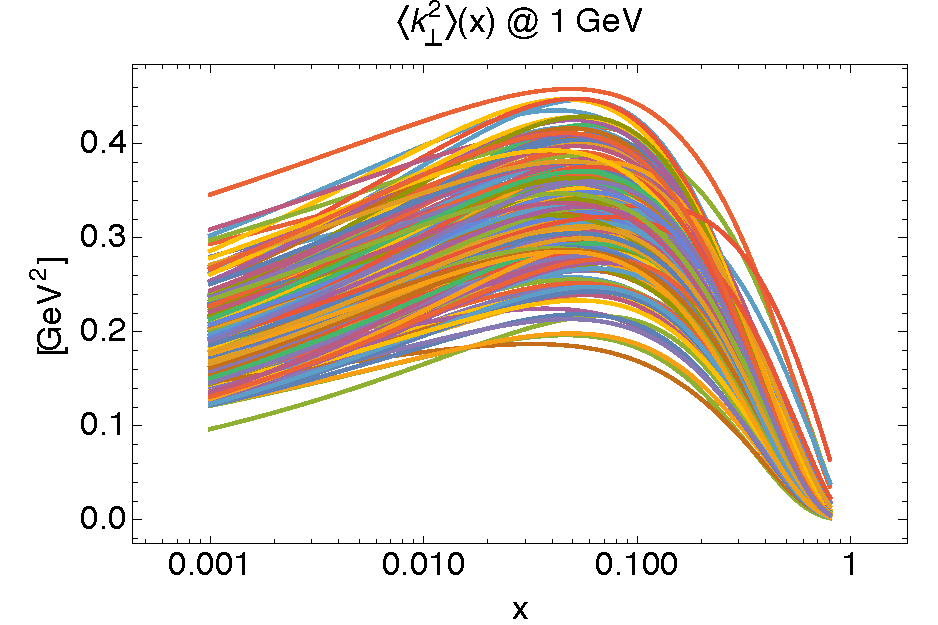
\includegraphics[width=0.40\textwidth]{plots/kT2av_curves_at1GeV_flINDEP.pdf}
&\hspace{0.001cm}
&
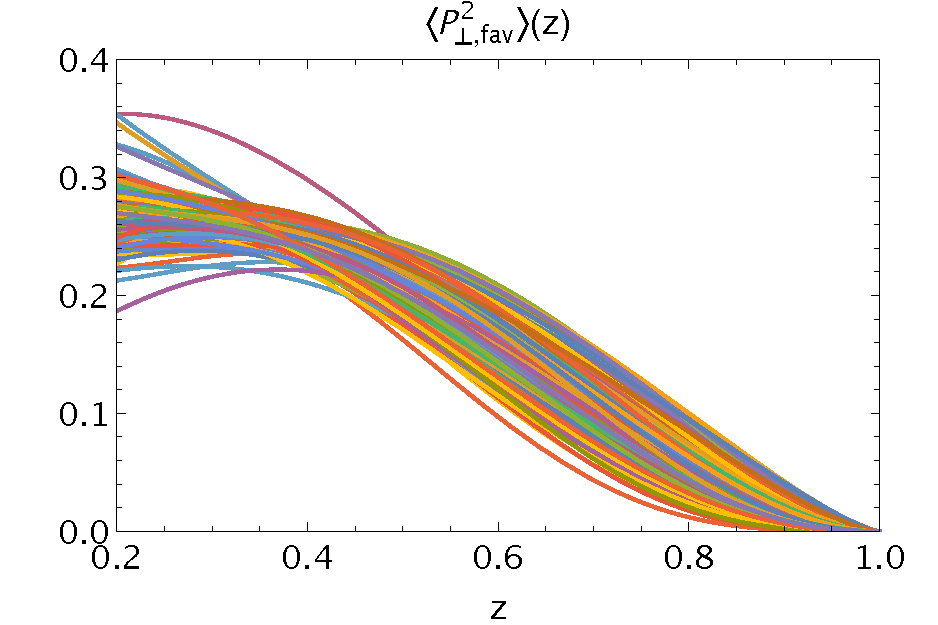
\includegraphics[width=0.40\textwidth]{plots/PT2av_curves_at1GeV_flINDEP.pdf}
\\
(a) && (b)
\end{tabular}
\caption{write the caption here (a) and another here (b).}
\label{f:avmomenta_all_rep}
\end{figure}
%%%%%%%%%%%%%%%%%%%%%%%%%%%%%%%%%
\begin{figure}[h!]
\centering
\begin{tabular}{ccc}
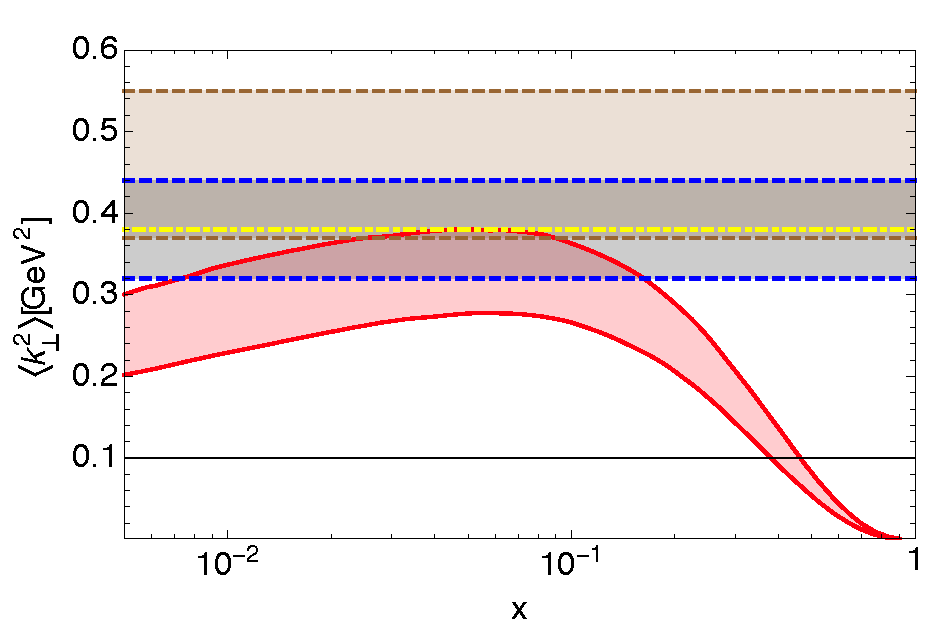
\includegraphics[width=0.40\textwidth]{plots/kT2av_Compare_with_other_extractions_flINDEP.pdf}
&\hspace{0.001cm}
&
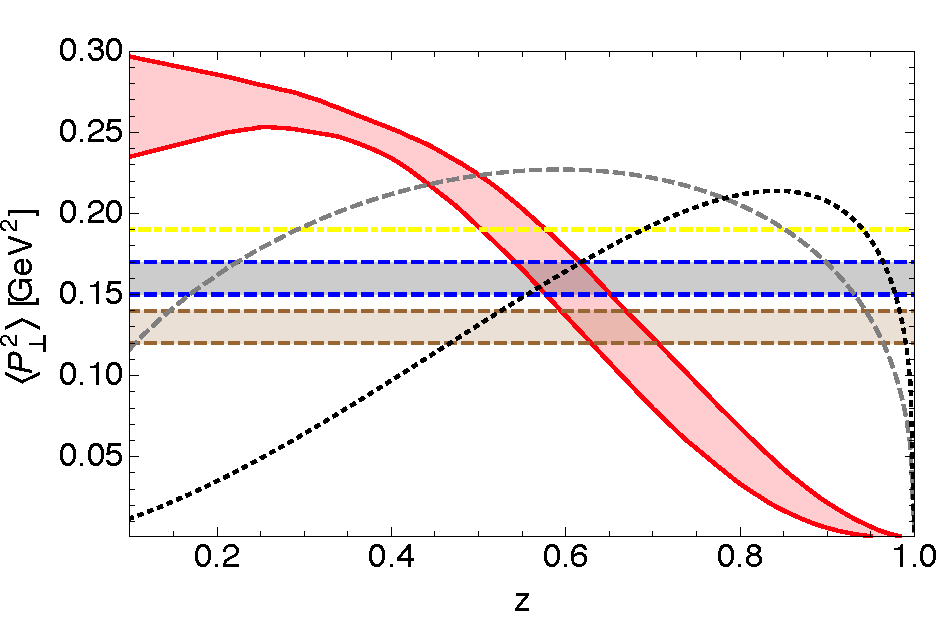
\includegraphics[width=0.40\textwidth]{plots/PT2av_Compare_with_other_extractions_flINDEP.pdf}
\\
(a) && (b)
\end{tabular}
\caption{write the caption here (a) and another here (b).}
\label{f:avmomenta_68CL}
\end{figure}
%%%%%%%%%%%%%%%%%%%%%%%%%%%%%%%%%







%\begin{table}[h]
%\small
%  \centering
%  \begin{tabular}{|c|c|c|c|c|c|c|c|c|c|}
%\hline
%\hline
%%  \multicolumn{4}{|c|}{Parameters for TMD PDFs} \\
%%  \hline
%%  \hline
%Points& Parameters & $\chi^2$& $\chi^2/$d.o.f.& 
%                  Points &$\chi^2$& Points &$\chi^2$& Points &$\chi^2$ 
% \\ 
%      &    &    &  & HERMES    & HERMES   & COMPASS & COMPASS & DY \& Z & DY \& Z  \\
%\hline
%8156 & 18  & $10456 \pm  $ & $1.28 \pm  $ & 1737&  &6126 & & 293 &    \\
%\hline
%\hline
%\end{tabular}
%\caption{Number of points and $\chi^2$ values 
%for the flavor-dependent fit}
%\label{t:chi2_flav}
%\end{table}
%
%\begin{table}
%\small
%  \centering
%  \begin{tabular}{|c|c|c|}
%\hline
%\hline
%%  \multicolumn{4}{|c|}{Parameters for TMD PDFs} \\
%%  \hline
%%  \hline
%$b_{\rm max}$ & $b_{\rm min}$ &  $g_2$ 
% \\ 
% (fixed)     & (fixed)   & {[GeV$^2$]}                           \\
%\hline
%$2 e^{-\gamma_E}/$GeV& $2 e^{-\gamma_E}/Q$  & $0.13 \pm 0.01$  \\
%\hline
%\hline
%\end{tabular}
%\caption{Values of parameters common to TMD PDFs and FFs 
%for the flavor-dependent fit}
%\label{t:parcommon_flav}
%\end{table}
%
%
%
%\begin{table}
%\small
%  \centering
%  \begin{tabular}{|c||c|c|c|c|c|c|}
%\hline
%\hline
%%  \multicolumn{4}{|c|}{Parameters for TMD PDFs} \\
%%  \hline
%%  \hline
%TMD PDFs&  $\big \langle \hat{\bm{k}}_{\T}^2 \big \rangle$ 
%& $\alpha$ & $\sigma$ & & $\lambda$ &  
% \\ 
%        & {[GeV$^2$]}                               &
%      (random) &      &  & & \\
%\hline
%up valence 
%& $0.15 \pm  $ & $0.00 \pm   $ & $-0.93 \pm  $  &  & $50.0 \pm  $ &
%\\
%\hline
%down valence 
%& $0.31 \pm  $ & '' & ''  &  & '' &    \\
%\hline
%sea 
%& $0.17 \pm  $ & $4.56 \pm   $ & $0.27 \pm  $  &  & $0.147 \pm  $ &    \\
%\hline
%\hline
%TMD FFs&  $\big \langle \hat{\bm{P}}_{\perp}^2 \big \rangle$ &
%$\beta$ & $\delta$ & $\gamma$ & $\lambda_F$ & $\big \langle
%\hat{\bm{P}}_{\perp}^{\prime 2} \big \rangle$
% \\ 
%        & {[GeV$^2$]} &            &         & & &{[GeV$^2$]}    \\
%\hline
%$u \to \pi^+$   &  $0.22 \pm $ & $2.6 \pm  $ & $2.8 \pm $ 
%      & $0.062 \pm $ & $5.9 \pm $ & $0.139 \pm $  \\
%\hline
%$d \to \pi^+$  &  $0.24 \pm $ & '' & '' & '' & '' & ''  \\
%\hline
%$\bar{s} \to K^+$ &  $0.24 \pm$ (random) & '' & '' & '' & '' & ''   \\
%\hline
%$u \to K^+$   &  $0.22 \pm $ & '' & '' & '' & '' & ''  \\
%\hline
%\hline
%\end{tabular}
%\caption{68\% confidence intervals of 
%best-fit parameters for TMD PDFs for the flavor-dependent fit}
%\label{t:fd_PDFs_par_flav}
%\end{table}







Description of Hermes data (version from Dropbox, Feb. 9$^{th}$).
Legend for $z$ values needs to be added too.
%%%%%%%%%%%%%%%%%%%%%%%%%%%%%%%%%
\begin{figure}[h!]
\begin{center}
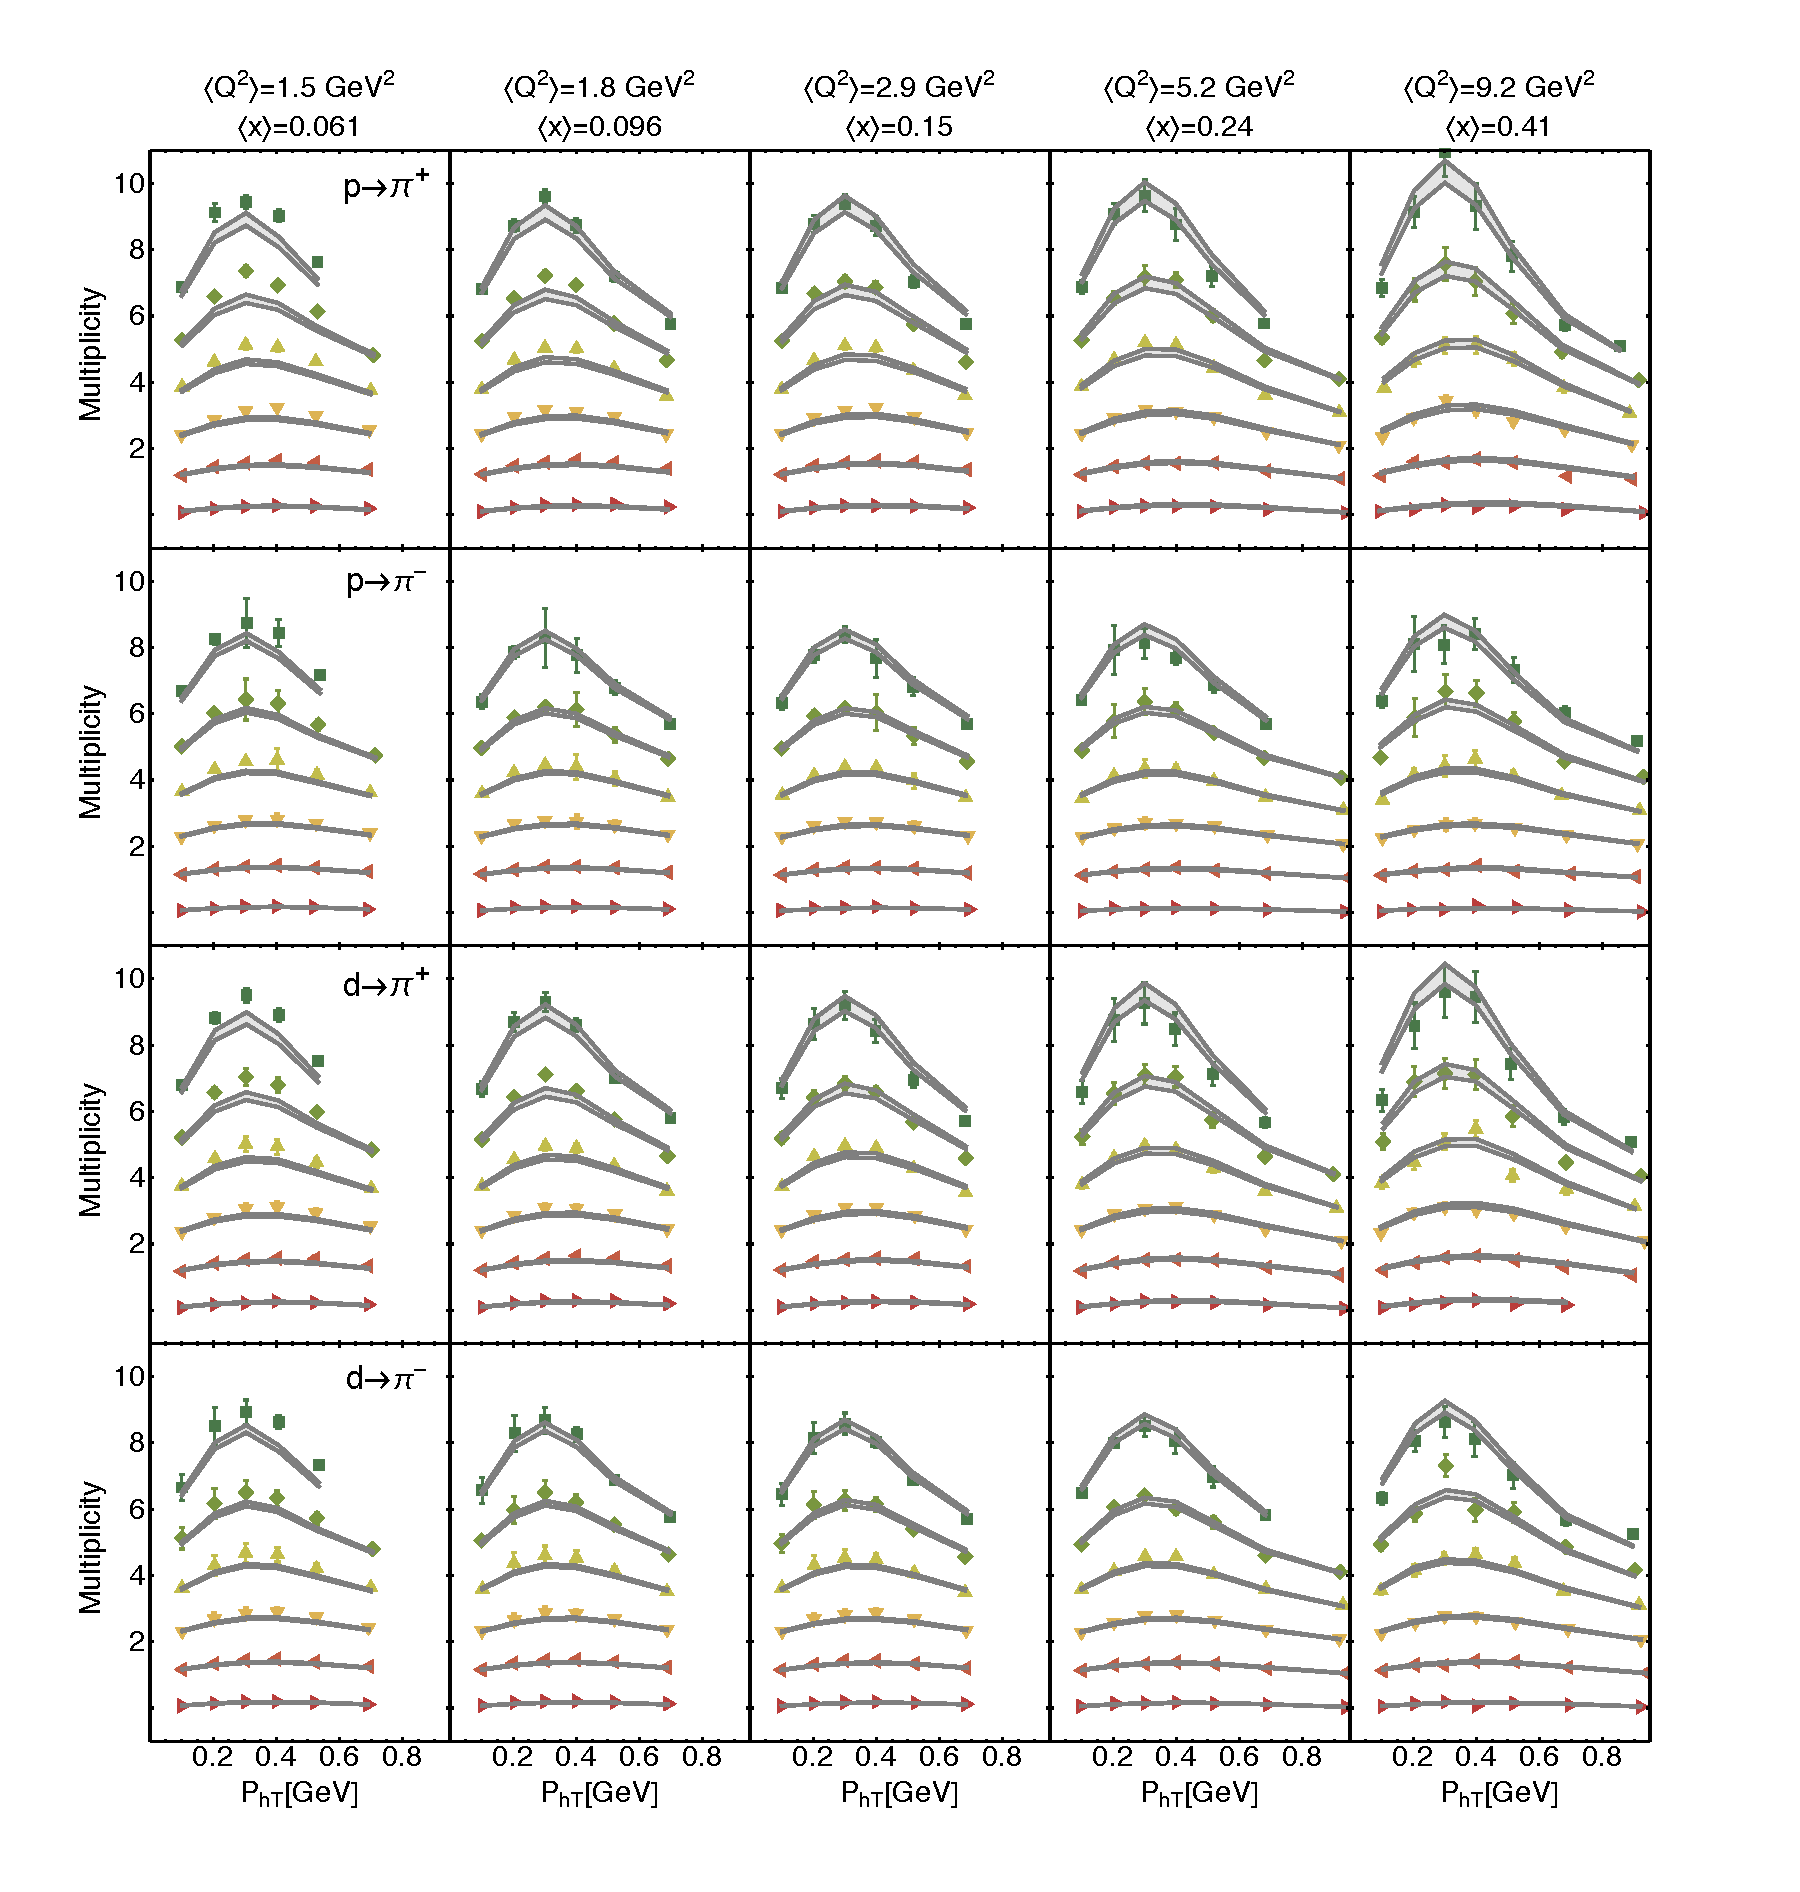
\includegraphics[width=0.95\textwidth]{plots/Hermes_Pions_SCIplot_flINDEP.pdf}
\end{center}
\caption{Hermes multiplicities for production of pions off a proton and a deuteron for different $\langle x \rangle$, $\langle z \rangle$, and $\langle Q^2 \rangle$ bins as a funciton of the transverse momentum of the dected hadron ${\bm P}_{hT}^ 2$.} 
\label{f:H_pions}
\end{figure}
%%%%%%%%%%%%%%%%%%%%%%%%%%%%%%%%%
\begin{figure}[h!]
\begin{center}
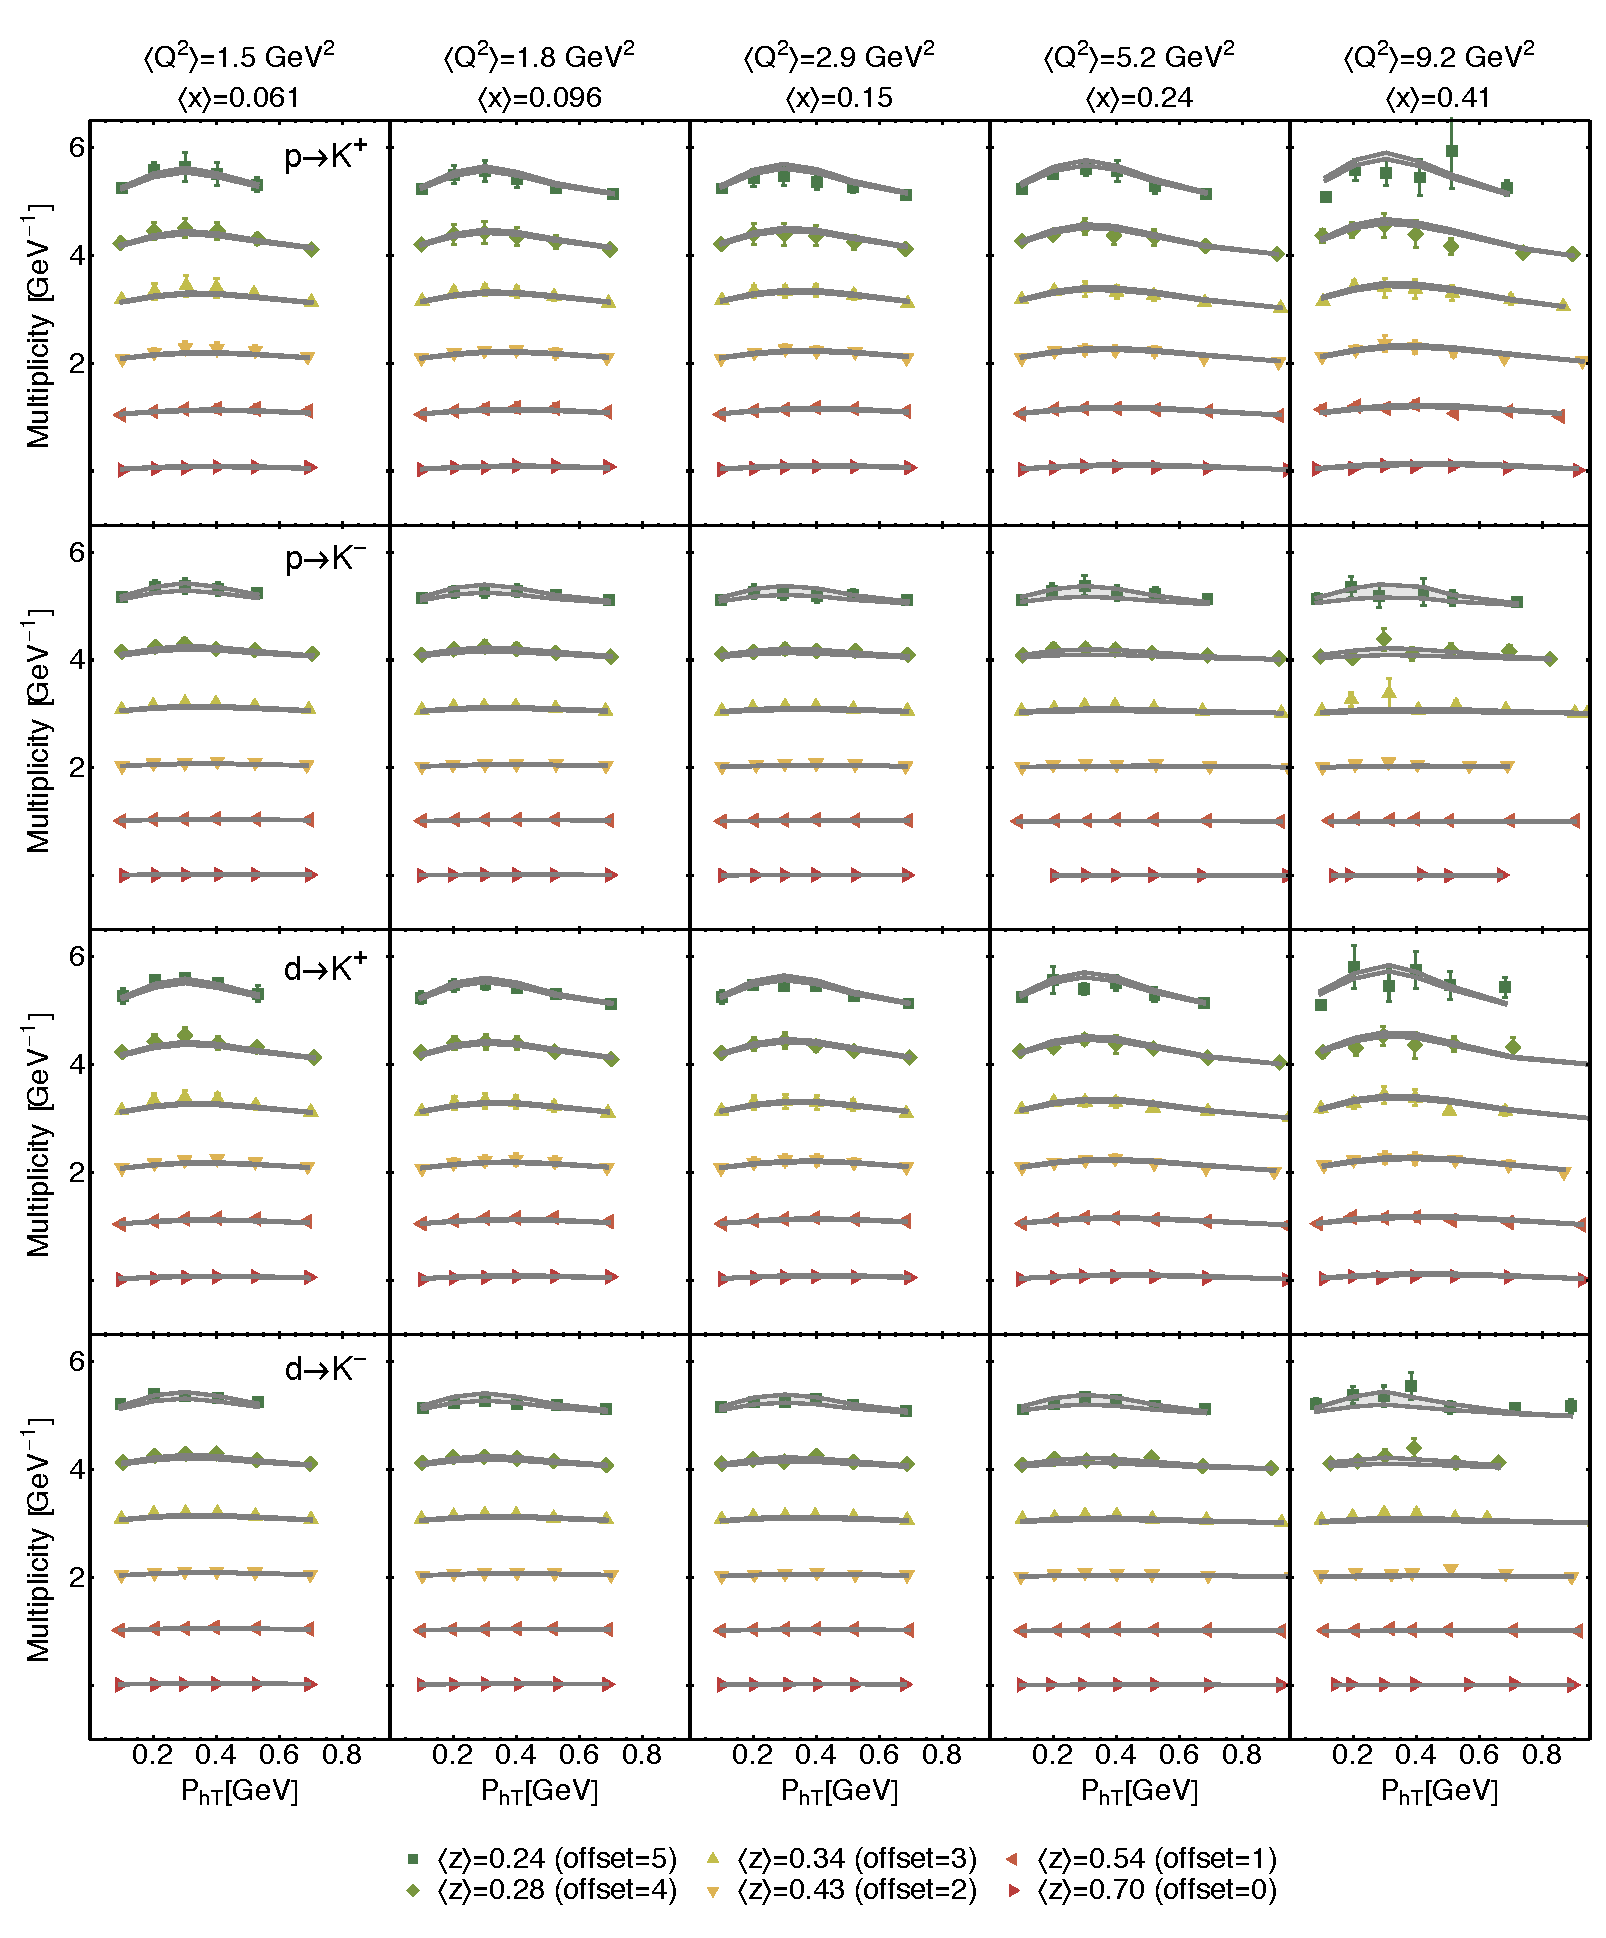
\includegraphics[width=0.95\textwidth]{plots/Hermes_Kaons_SCIplot_flINDEP.pdf}
\end{center}
\caption{Hermes multiplicities for production of kaons off a proton and a deuteron for different $\langle x \rangle$, $\langle z \rangle$, and $\langle Q^2 \rangle$ bins as a funciton of the transverse momentum of the dected hadron ${\bm P}_{hT}^ 2$.} 
\label{f:H_kaons}
\end{figure}
%%%%%%%%%%%%%%%%%%%%%%%%%%%%%%%%%



Description of Compass data (version from Dropbox, Feb. 9$^{th}$).
%%%%%%%%%%%%%%%%%%%%%%%%%%%%%%%%%
\begin{figure}[h!]
\begin{center}
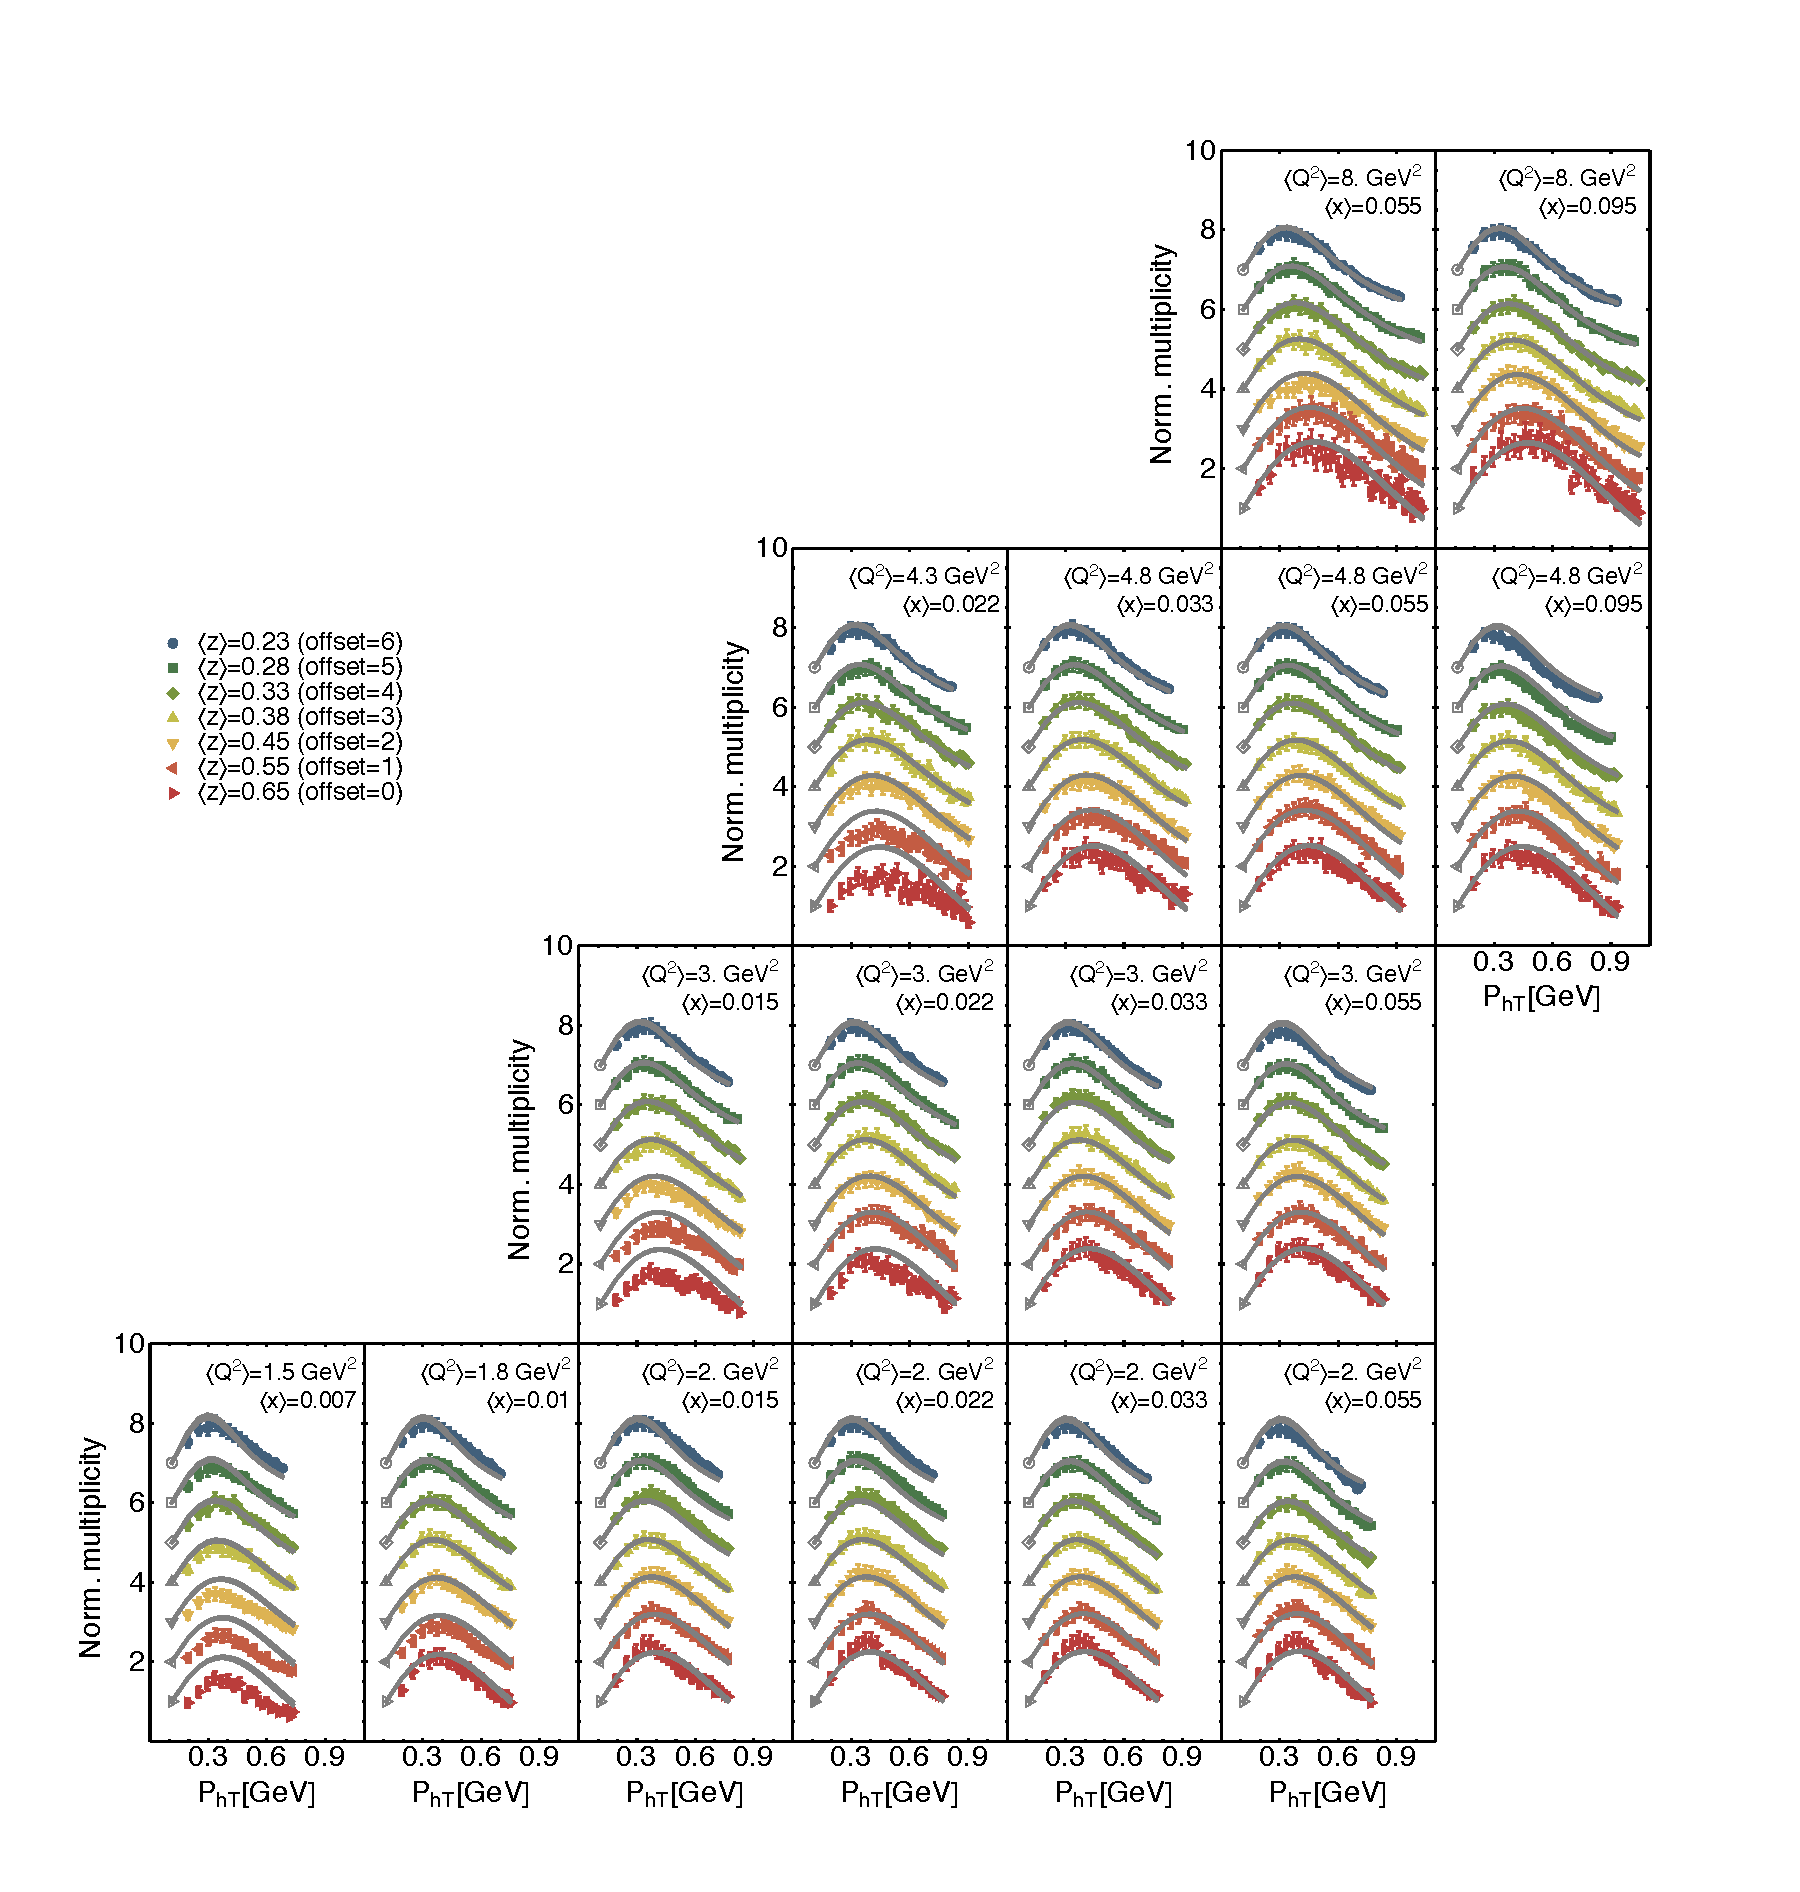
\includegraphics[width=\textwidth]{plots/COMPASS_SCIplot_flINDEP_Piminus.pdf}
\end{center}
\caption{Compass multiplicities for production of negative hadrons (pions) off a deuteron for different $\langle x \rangle$, $\langle z \rangle$, and $\langle Q^2 \rangle$ bins as a funciton of the transverse momentum of the dected hadron ${\bm P}_{hT}^ 2$. Multiplicities are normalized to the first bin in ${\bm P}_{hT}^ 2$ for each $\langle z \rangle$ value.} 
\label{f:C_pim}
\end{figure}
%%%%%%%%%%%%%%%%%%%%%%%%%%%%%%%%%
\begin{figure}[h!]
\begin{center}
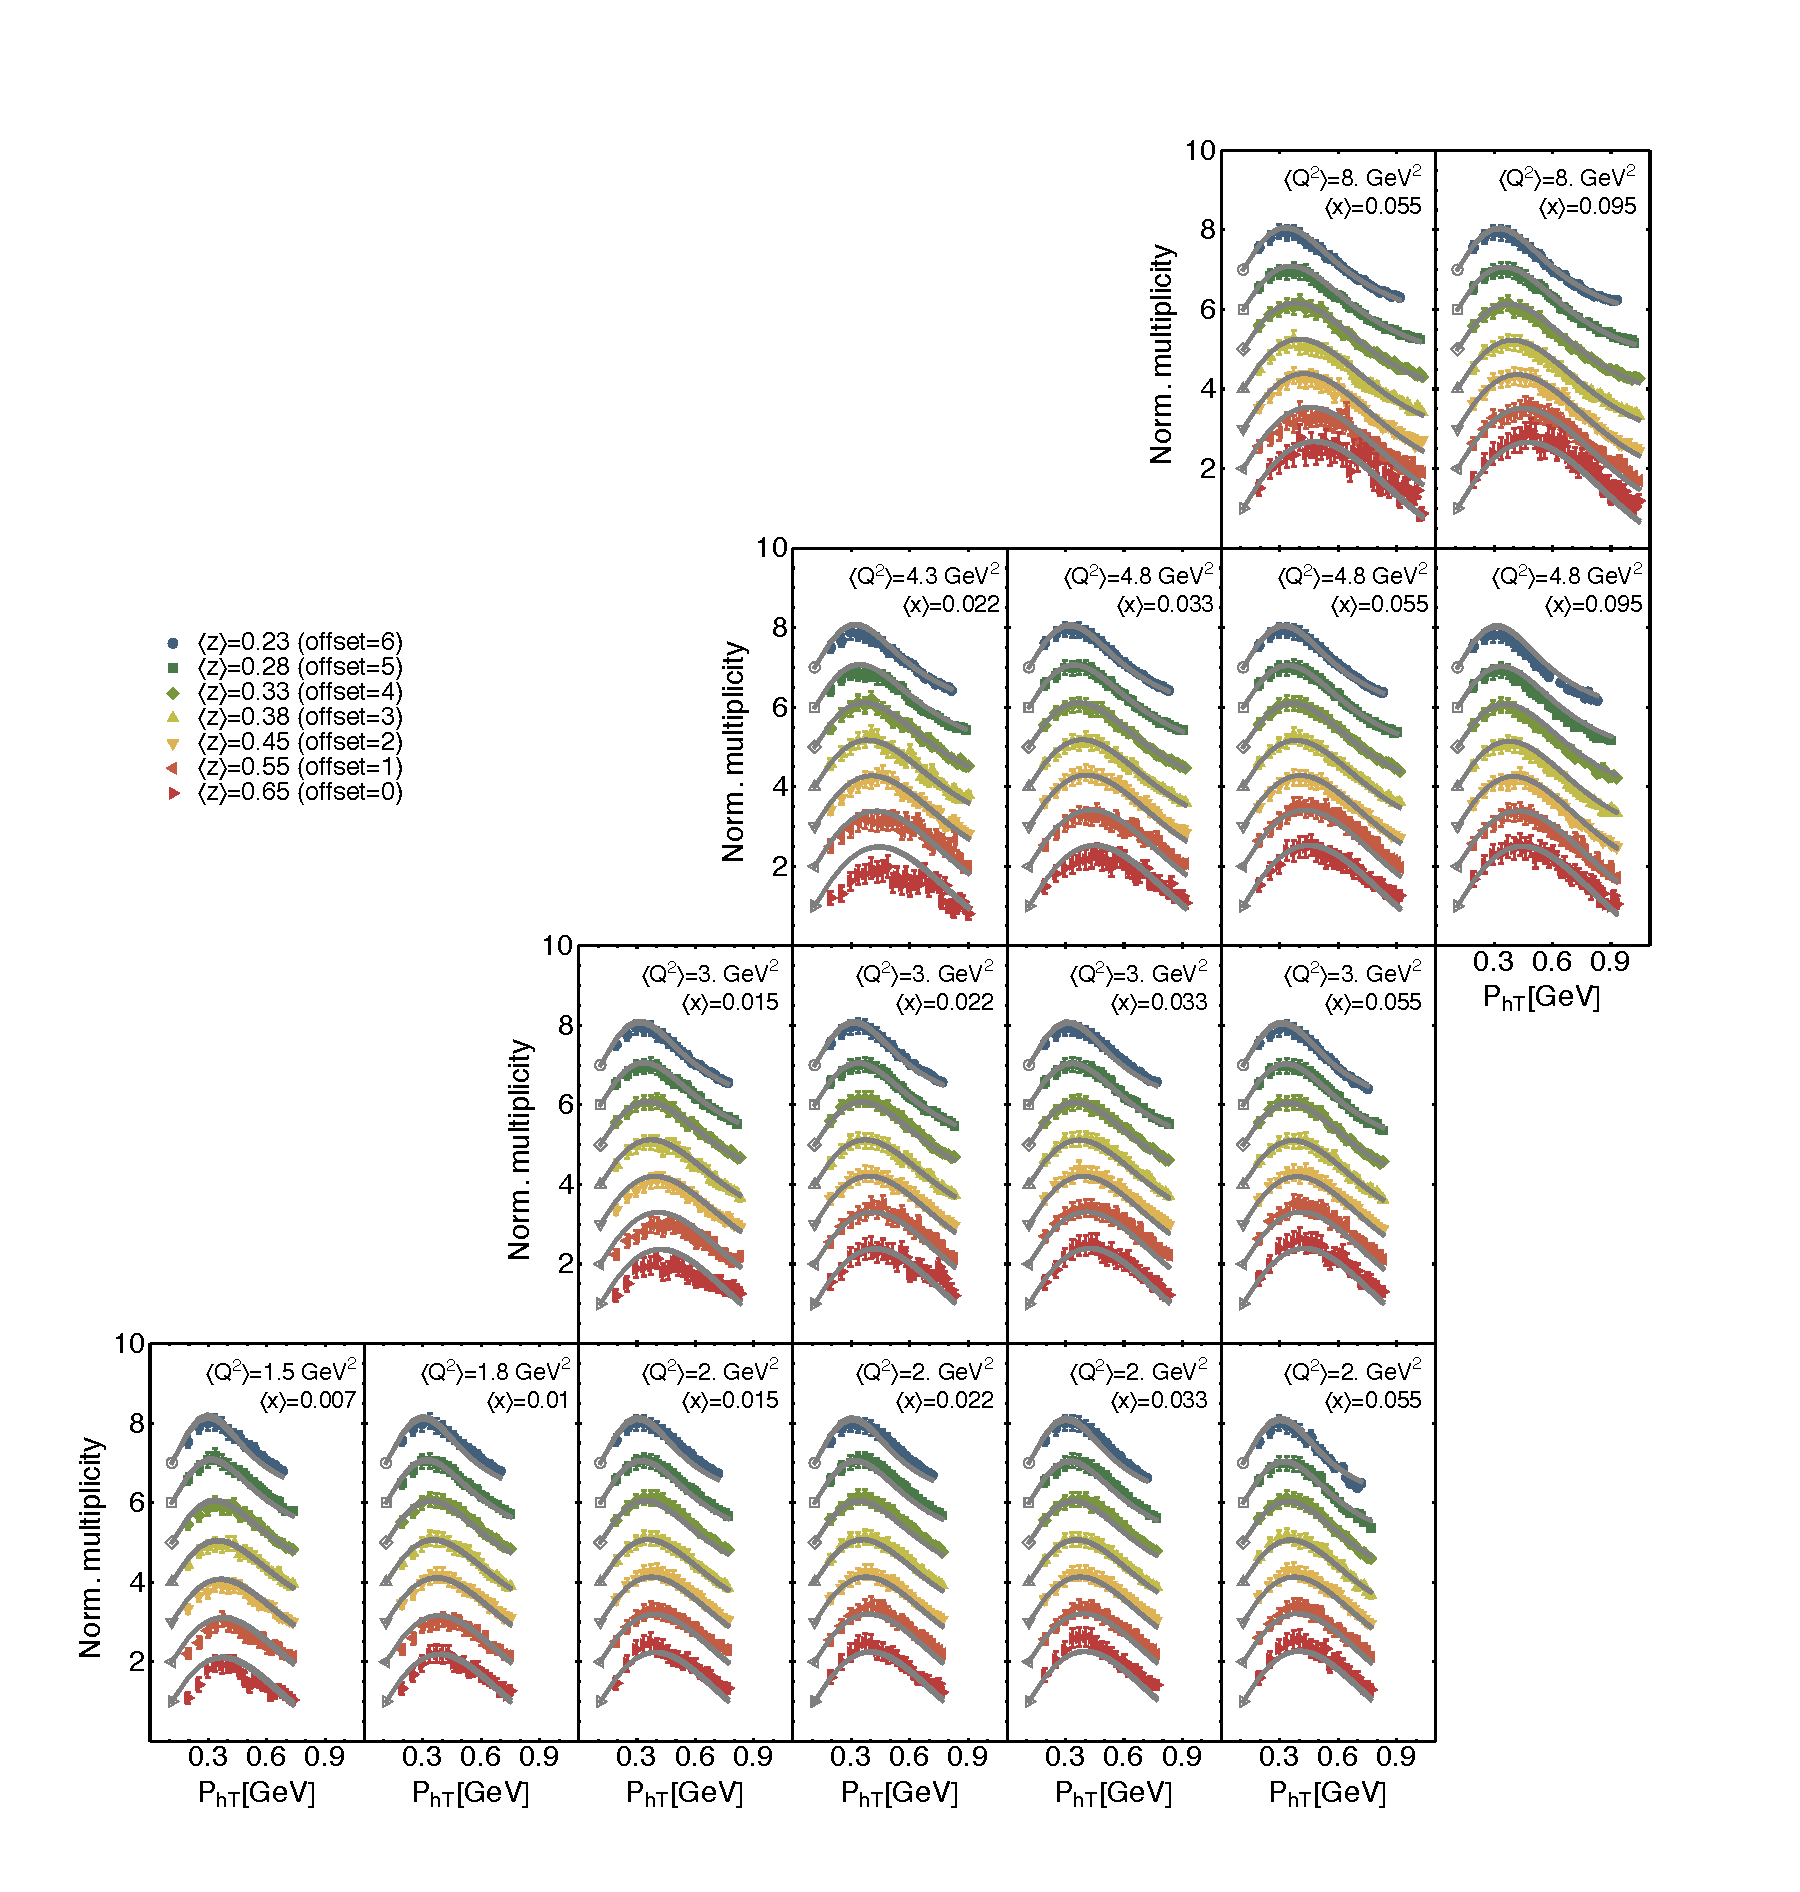
\includegraphics[width=\textwidth]{plots/COMPASS_SCIplot_flINDEP_Piplus.pdf}
\end{center}
\caption{Compass multiplicities for production of positive hadrons (pions) off
  a deuteron for different $\langle x \rangle$, $\langle z \rangle$, and
  $\langle Q^2 \rangle$ bins as a funciton of the transverse momentum of the
  dected hadron ${\bm P}_{hT}^ 2$. Multiplicities are normalized to the first
  bin in ${\bm P}_{hT}^ 2$ for each $\langle z \rangle$ value. For clarity,
  each $\langle z \rangle$  bin has been shifted by an offset indicated in the legend.} 
\label{f:C_pip}
\end{figure}
%%%%%%%%%%%%%%%%%%%%%%%%%%%%%%%%%





Description of low energy Drell-Yan data (version from Dropbox, Feb. 9$^{th}$).
Legends need to be added too. Fix the y-axis label.
%%%%%%%%%%%%%%%%%%%%%%%%%%%%%%%%%%
\begin{figure}[h!]
\centering
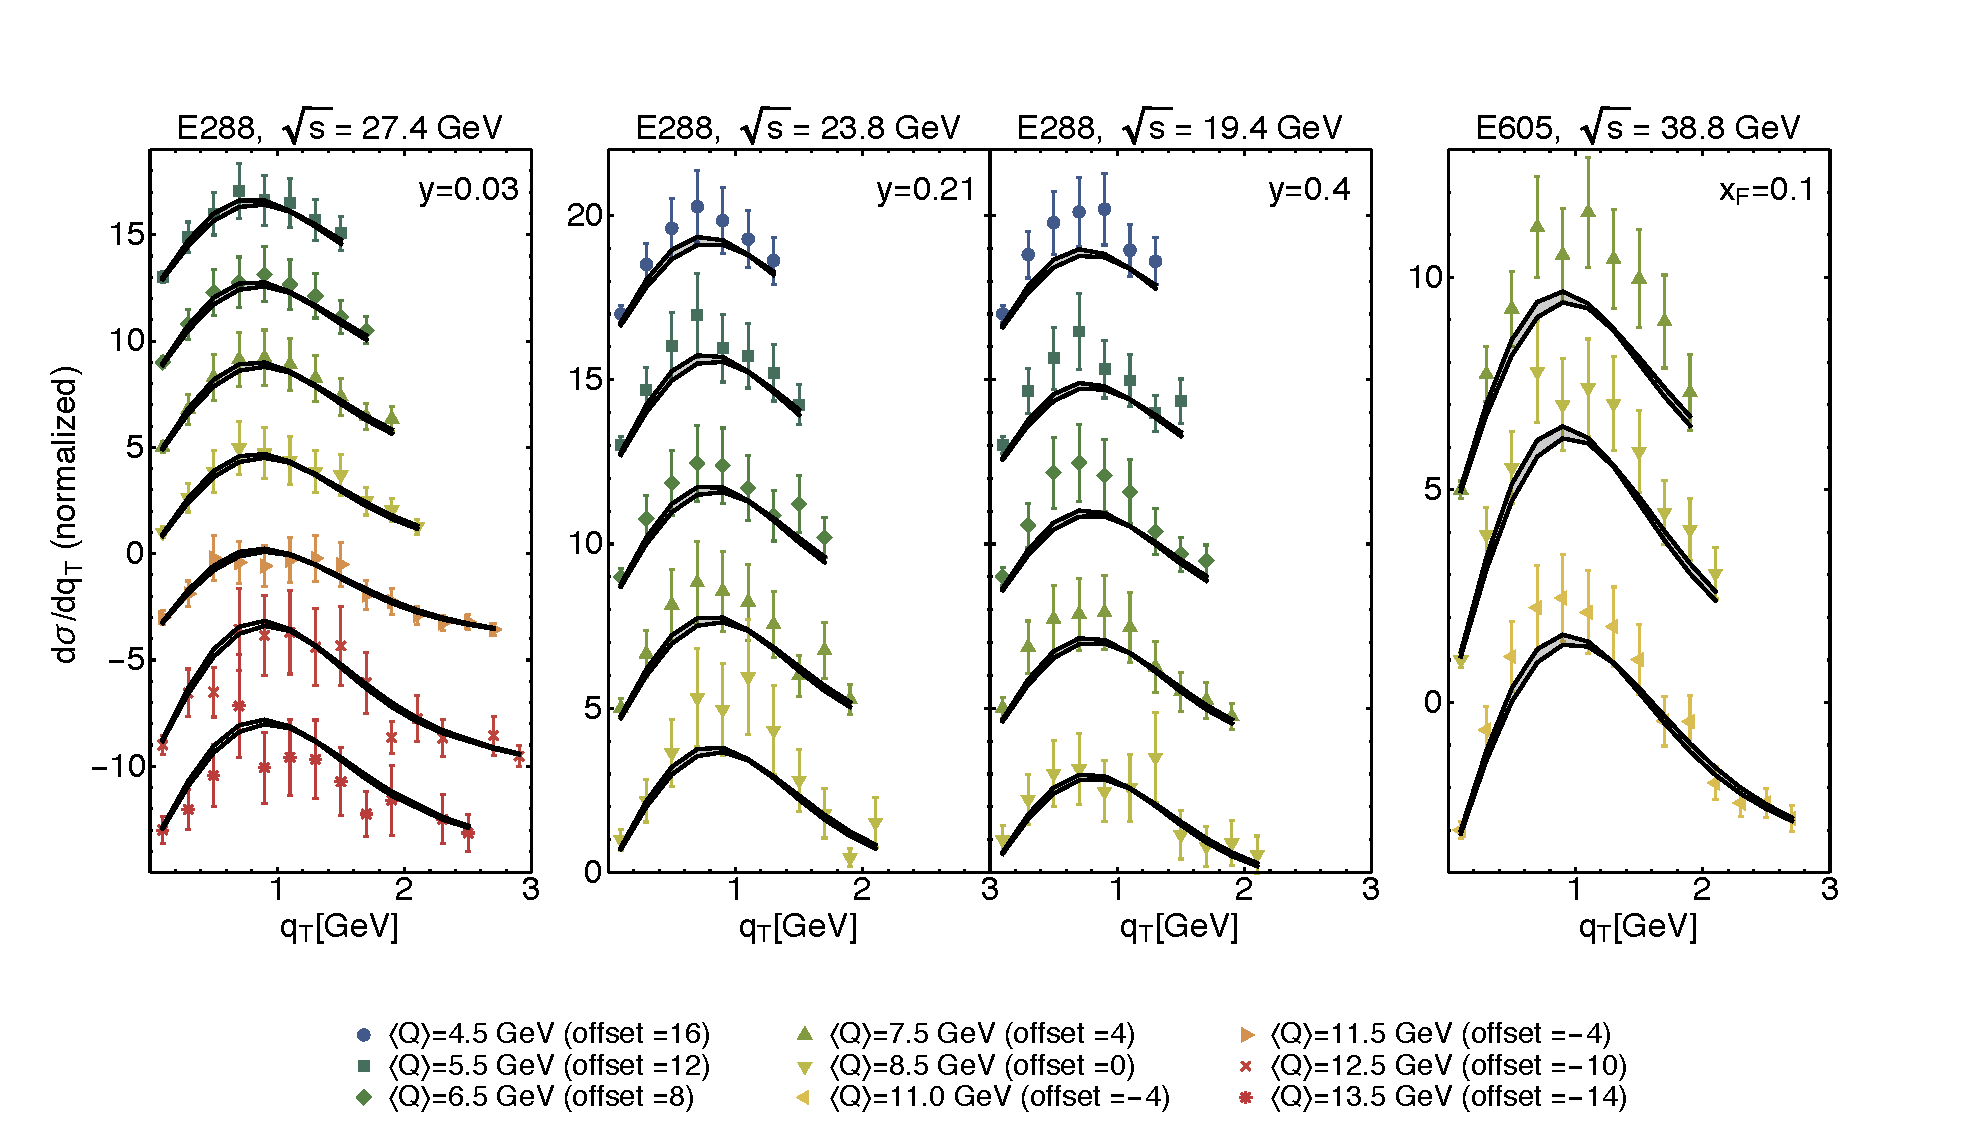
\includegraphics[width=0.95\textwidth]{plots/DY_SCIplot_flINDEP.pdf}
\caption{Drell-Yan differential cross section for different experiments and
  different values of $\sqrt{s}$ and for different $\langle Q \rangle$ bins.
  For clarity, each $\langle A \rangle$  bin has been shifted by an offset
  indicated in the legend.}
\label{f:DY_panel}
\end{figure}
%%%%%%%%%%%%%%%%%%%%%%%%%%%%%%%%%
%%%%%%%%%%%%%%%%%%%%%%%%%%%%%%%%%%
%\begin{figure}[h!]
%\centering
%\begin{tabular}{ccc}
%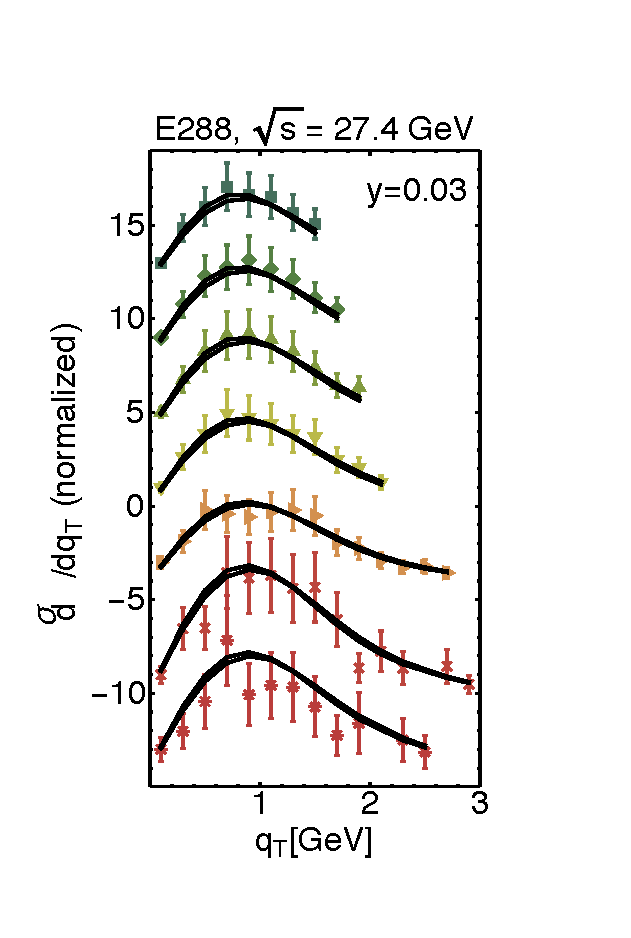
\includegraphics[width=0.40\textwidth]{plots/DY_SCIplot_flINDEP_1.pdf}
%&\hspace{0.001cm}
%&
%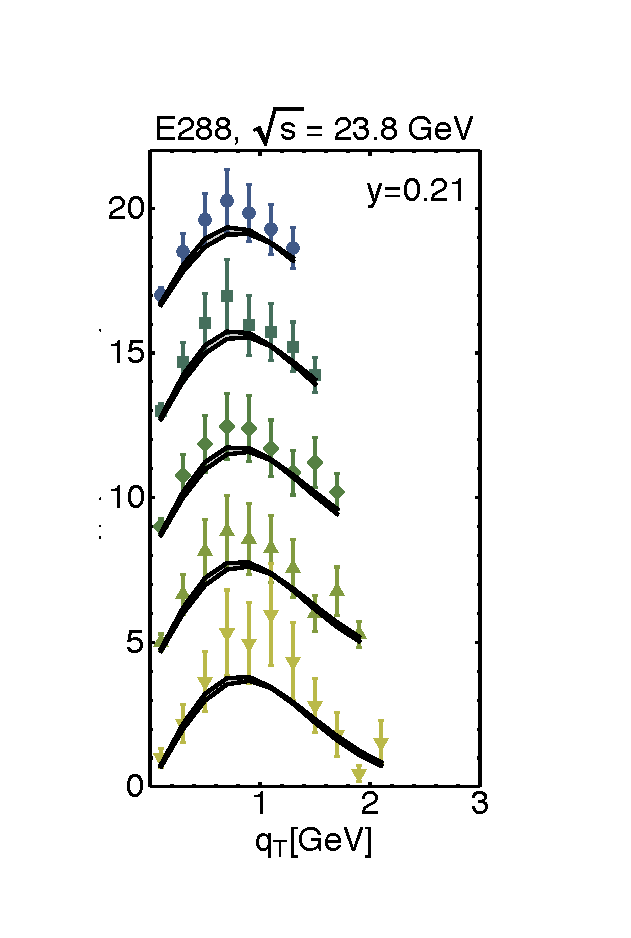
\includegraphics[width=0.40\textwidth]{plots/DY_SCIplot_flINDEP_2.pdf}
%\\
%(a) && (b)
%\end{tabular}
%\caption{write the caption here (a) and another here (b).}
%\label{f:DY_panel_1}
%\end{figure}
%%%%%%%%%%%%%%%%%%%%%%%%%%%%%%%%%%
%\begin{figure}[h!]
%\centering
%\begin{tabular}{ccc}
%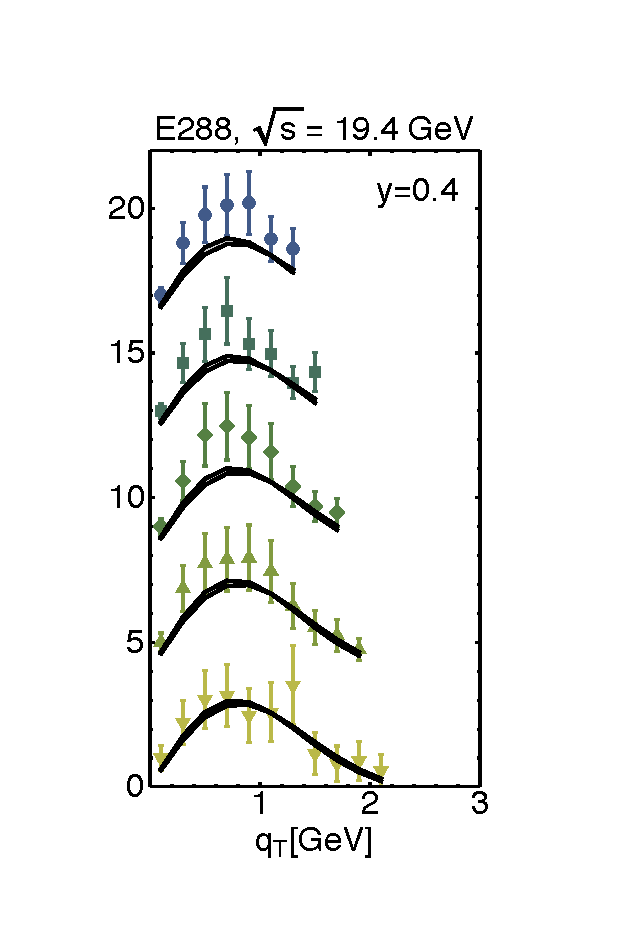
\includegraphics[width=0.40\textwidth]{plots/DY_SCIplot_flINDEP_3.pdf}
%&\hspace{0.001cm}
%&
%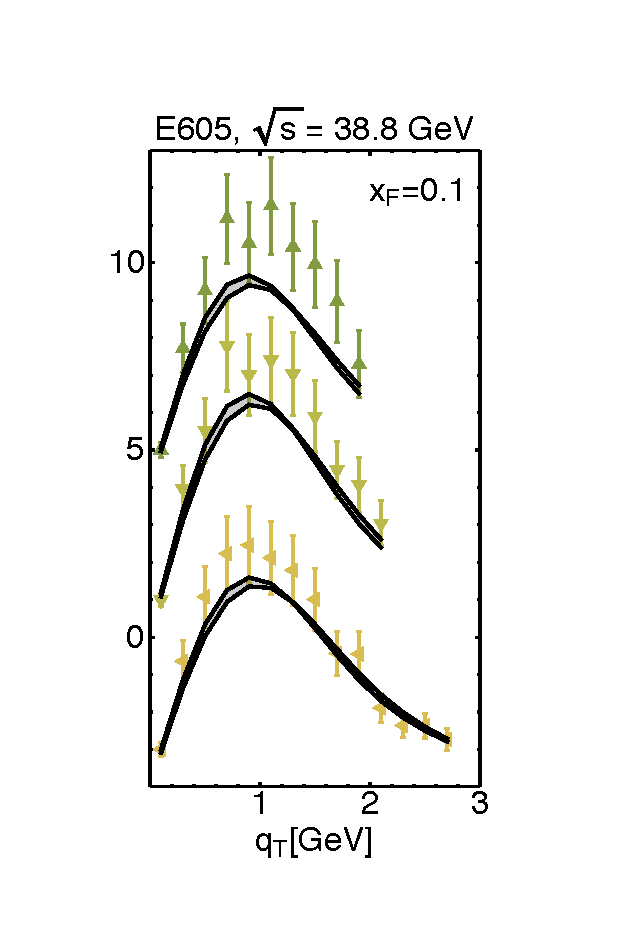
\includegraphics[width=0.40\textwidth]{plots/DY_SCIplot_flINDEP_4.pdf}
%\\
%(a) && (b)
%\end{tabular}
%\caption{write the caption here (a) and another here (b).}
%\label{f:DY_panel_2}
%\end{figure}
%%%%%%%%%%%%%%%%%%%%%%%%%%%%%%%%%%
%
%
%


Description of Z-boson production data (version from Dropbox, Feb. 9$^{th}$).
Legends need to be added too. Fix the y-axis label.
%%%%%%%%%%%%%%%%%%%%%%%%%%%%%%%%%
\begin{figure}[h!]
\begin{center}
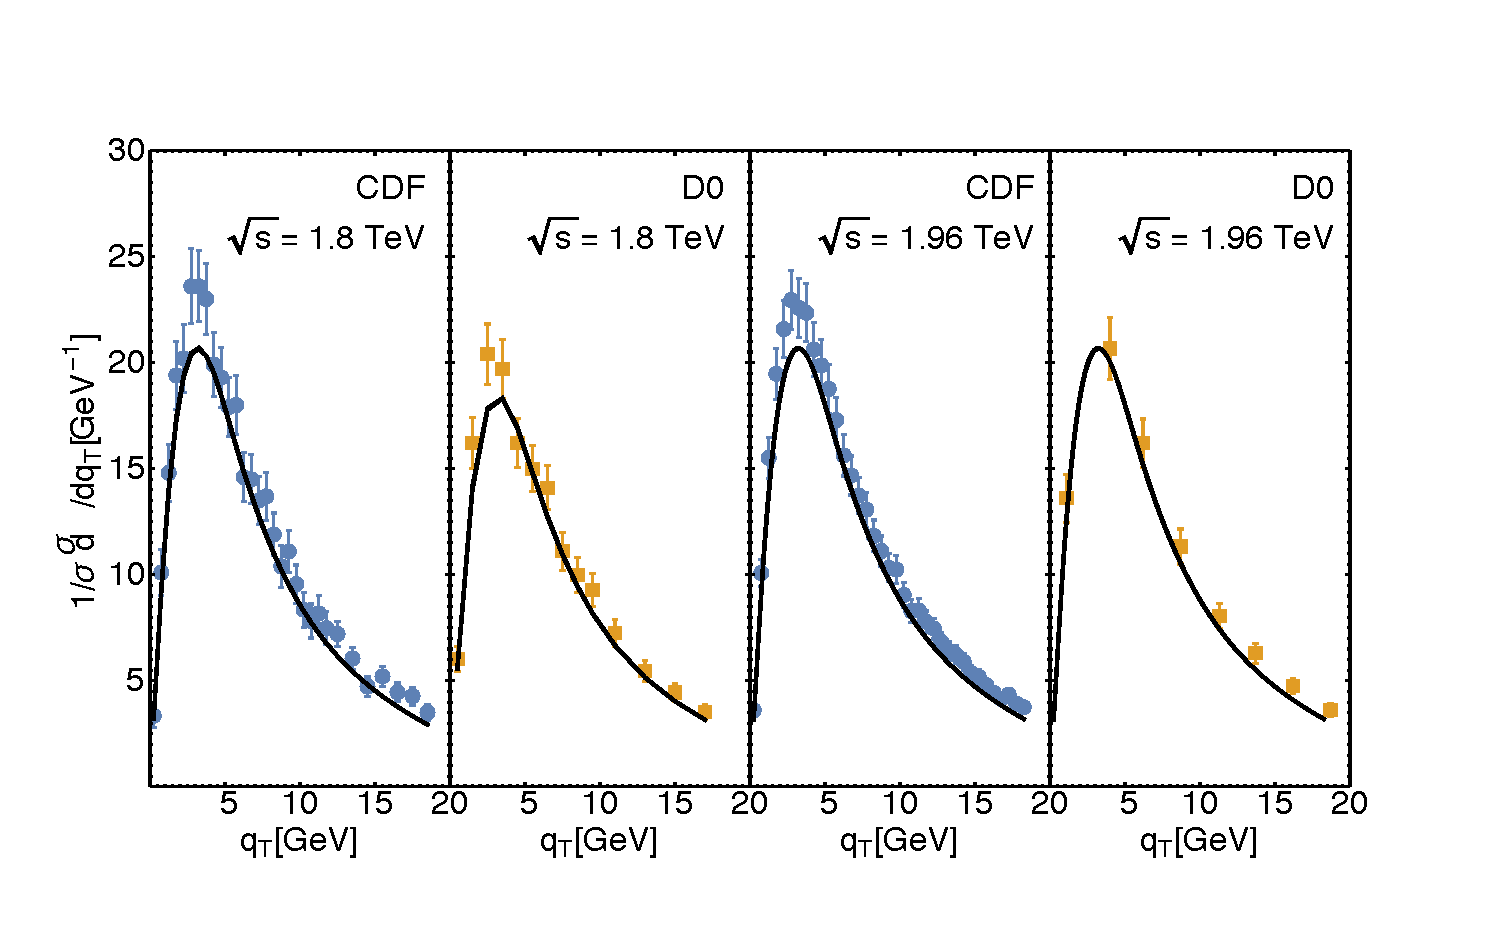
\includegraphics[width=0.95\textwidth]{plots/Z_SCIplot_flINDEP.pdf}
\end{center}
\caption{Cross section differential with respect to the transverse momentum $q_T$ of a $Z$ boson produced from $p\bar{p}$ collisions at Tevatron. The four panels refer to different experiments (CDF and D$0$) with two different values for the center-of-mass energy ($\sqrt{s} = 1.96$ TeV and $\sqrt{s}=1.8$ TeV).} 
\label{f:Z_qT}
\end{figure}
%%%%%%%%%%%%%%%%%%%%%%%%%%%%%%%%%











%%%%%%%%%%%%%%%%%%%%%%%%%%%%%%%%%%%%%%%%%%%%%%%%%%%%%%%%%%%%%%%%%%
\section{Conclusions and outlook}
\label{s:end}
%%%%%%%%%%%%%%%%%%%%%%%%%%%%%%%%%%%%%%%%%%%%%%%%%%%%%%%%%%%%%%%%%%



\newpage
%%%%%%%%%%%%%%%%%%%%%%%%%%%%%%%%%%%%%%%%%%%%%%%%%%%%%%%%%%%%%%%%%%
\begin{acknowledgments}
%Discussions with  are gratefully acknowledged. 
This work is supported by the European Research Council (ERC) under the European Union's Horizon 2020 research and innovation program (grant agreement No. 647981, 3DSPIN). 
AS acknowledges support from U.S. Department of Energy contract DE-AC05-06OR23177, under which Jefferson Science Associates, LLC, manages and operates Jefferson Lab. 
The work of AS has been funded partly also by the program of the Stichting voor Fundamenteel Onderzoek der Materie (FOM), which is financially supported by the Nederlandse Organisatie voor Wetenschappelijk Onderzoek (NWO).
\end{acknowledgments}
%%%%%%%%%%%%%%%%%%%%%%%%%%%%%%%%%%%%%%%%%%%%%%%%%%%%%%%%%%%%%%%%%%
%\bibliographystyle{myrevtex}
%\bibliographystyle{h-physrev}
\bibliographystyle{apsrevM}
%\bibliographystyle{JHEP}
\bibliography{mybiblio}
%\bibliography{biblio_sidis}
%\bibliography{bibroad}
%%%%%%%%%%%%%%%%%%%%%%%%%%%%%%%%%%%%%%%%%%%%%%%%%%%%%%%%%%%%%%%%%%


\end{document}

%%% Local Variables: 
%%% mode: latex
%%% TeX-master: t
%%% End: 


%% figure with one panel :
%%%%%%%%%%%%%%%%%%%%%%%%%%%%%%%%%
%\begin{figure}[h!]
%\begin{center}
%\includegraphics[width=***cm]{fig_name}
%\end{center}
%\caption{} 
%\label{f:xxxxx}
%\end{figure}
%%%%%%%%%%%%%%%%%%%%%%%%%%%%%%%%%

%%% figure with two panels :
%%%%%%%%%%%%%%%%%%%%%%%%%%%%%%%%%%
%\begin{figure}
%\centering
%\begin{tabular}{ccc}
%\includegraphics[width=***cm]{fig_name}
%&\hspace{0.001cm}
%&
%\includegraphics[width=6cm]{fig_name}
%\\
%(a) && (b)
%\end{tabular}
%\caption{write the caption here (a) and another here (b).}
%\label{f:xxxxx}
%\end{figure}
%%%%%%%%%%%%%%%%%%%%%%%%%%%%%%%%%




